% #############################################################################
% This is Chapter 5
% !TEX root = main.tex
% #############################################################################
% Change the Name of the Chapter i the following line
\fancychapter{Assessment of Intelligent Agents}
\clearpage
% The following line allows to ref this chapter
\label{chap:chap005}

In the last chapter (Chapter~\ref{chap:chap004}), the thesis introduces the development of a framework (Section~\ref{sec:sec004003}).
Indeed, this framework will serve as the basis of the main work objectives (Section~\ref{sec:sec001002}).
Consequently, the first steps for the design of a labeling tool (Section~\ref{sec:sec004003002}) are made.
For medical imaging annotations, the tool is promoting a standardized generation of datasets (Section~\ref{sec:sec004004002}) which will fulfil the thesis main concerns.
After all, the datasets are important information to train the implemented models.

A proof-of-concept tool was designed for the production of qualified datasets in order to provide clinicians, as well as the \ac{ML} community, a sharing and collaborative solution (Section~\ref{sec:sec004002003}).
This solution is giving the potential to extract features (Section~\ref{sec:sec002006}), like contours, intersections, margins, shapes and severities that can be used in the process of lesion segmentation and classification.
As a result of that, the framework is covering the initial challenges (Section~\ref{sec:sec001002}) concerning the lack of available and curated medical data.
Due to a human-centered approach, the annotating process is now enabling clinicians to understand the importance between existing medical data and \ac{AI} algorithms.
However, this is just a minor concern according to the main objectives of this thesis.

For this thesis, the main goal is to understand how the implemented \ac{DL} methods (Section~\ref{sec:sec003007}) can consume the aforementioned generated data and being integrated within an intelligent agent.
Moreover, it is of chief importance to understand how the intelligent agent(s) can better communicate with clinicians as a second reader.
In this chapter, the document takes a \ac{HCI} perspective on the opportunities provided by \ac{AI} techniques in medical imaging, focusing on workflow efficiency and quality, preventing errors and variability of diagnosis in breast cancer.

\section{Introduction}
\label{sec:sec005001}

\ac{AI} has the potential to fundamentally transform many application domains~\cite{ghahramani2015probabilistic}.
One notable example is clinical radiology \cite{choy2018current, hosny2018artificial}, for which a growing number of \ac{AI}-based systems have been proposed for lesion detection and segmentation.
In the \ac{RRR}, these are two fundamental steps to accomplish the diagnosis and treatment planning \cite{kooi2017large, graffy2019automated, lakhani2017deep, liang2019deep}.
This synergy between \ac{AI} and medical imaging is currently known as {\it radiomics}~\cite{Lambin2017} and aims to develop methods that automatically analyze large amounts of data and extract meaningful features to support diagnosis~\cite{Ruddle:2016:DEI:2872314.2834117} and clinical decision making~\cite{Park:2015:TOA:2737795.2656213}.

Many studies have reported robust and relevant findings in {\it radiomics}~\cite{aerts2017data}.
Without hand-designed features~\cite{ker2018deep}, the field is including significant hierarchical relationships within the data automatically discovered.
However, a growing number of these studies also suffer from deficient experimental or analytic designs~\cite{aerts2017data}.
Thus, failing to include a more holistic understanding of the clinical context~\cite{Sultanum:2018:MTP:3173574.3173996}.
While \ac{AI} is changing the paradigm both in terms of visualization and interaction in the {\it radiomics} workflow, it is still not clear neither how it influences radiologists, nor what is the best approach to maximize the benefits of this Human-\ac{AI} collaboration \cite{Kocielnik:2019:YAI:3290605.3300641}.

Across the several clinical institutions\footnotemark[20], the goal of this chapter is to provide an assessment of the impact of intelligent agents on the diagnostic performance of radiologists.
The work focus on the breast screening problem, in which radiologists typically require multimodality (\ac{MG}, \ac{US} and \ac{MRI}) to detect suspicious regions (lesion) on the breast.
This multi-modal setup is very challenging, not only due to the large amount of data being processed, but also for manipulation and visualization of heterogeneous data.
To this end, under the chapter work it was developed the {\it BreastScreening-AI}, a multi-modal \ac{AI}-assisted framework  that allows the radiologist to view, manipulate and classify medical images in an effortless way, while also providing diagnostic recommendations.

%%%%%%%%%%%%%%%%%%%%%%%%%%%%%%%%%%%%%%%%%%%%%%%%%%%
\footnotetext[20]{The number of clinicians and institutions that supported the developed work are:
12 clinicians of Hospital Fernando Fonseca; % HFF
10 clinicians of IPO Lisboa; %IPOL
2 clinicians of Hospital Santa Maria; %HSM
9 clinicians of IPO Coimbra; %IPOC
1 clinician of Madeira Medical Center; and %MMC
1 clinician of Hospital SAMS; %SAMS
8 clinicians of Hospital do Barreiro; %HB
1 clinician of Hospital Santo Ant\'{o}nio; %HSA
1 clinician of Jo\~{a}o Carlos Costa Clinic. %JCC
This study collected the patient data from the first institution ({\it i.e.}, Hospital Fernando Fonseca).
Then, we applied our \ac{UTA} to the full list of clinical institutions and clinicians.
}
%%%%%%%%%%%%%%%%%%%%%%%%%%%%%%%%%%%%%%%%%%%%%%%%%%%

\subsection{Motivation}
\label{sec:sec005001001}

Breast cancer (Section~\ref{sec:sec002002}) is one of the most diagnosed cancers worldwide~\cite{desantis2016breast, torre2015global}.
In fact, breast cancer is the second leading cause of death from cancer in women~\cite{doi:10.3322/caac.21492}.
Early detection is one of the most effective ways to increase the survival rate for this disease~\cite{welch2016breast, saadatmand2015influence}.
Screening mammography aims to identify breast cancer at earlier stages of the disease, when treatment can be more successful~\cite{McKinney2020}.
However, two main difficulties arise.
First, the amount of data to be processed has been increasing significantly and greatly surpasses the throughput capabilities of the radiologists.
Second, processing such amount of multi-modal data (Figure~\ref{fig:fig005}) in timely fashion without compromising the reliability of the diagnosis which is very challenging.
These difficulties have been the driving force behind the recent trend in {\it radiomics} (Section~\ref{sec:sec002006}) and the integration of \ac{AI} techniques into medical imaging.

Agent-based tools are one of the new paradigm for complex and distributed healthcare systems~\cite{10.1145/3206505.3206555, esteva2019guide}.
In this paradigm, developed components are not tightly coupled with one another and can work autonomously, even in unpredictable environments.
Intelligent agents are the natural choice for dynamic and critical environments that are characterized with heterogeneous information and its interactions, rapidly growing data quantity and different data representation forms, such as segmentation and classification of lesions.
Hence, the use of these agents can provide additional value for the final diagnostic.

Support for visualization of multi-modal images and \ac{AI} techniques can provide improvements and insights in the breast screening radiology workflow (Section~\ref{sec:sec002005}).
In this chapter, the goal is to evaluate the impact of the integration of these techniques in the context of the breast cancer diagnosis using the {\it BreastScreening-AI} tool.
Specifically, this work focus on how multimodality and intelligent agents could add a value in the {\it radiomics} medical workflow~\cite{calisto2017mimbcdui}.
The answers of the work to this problem include usage and acceptance by physicians and the improvement of workflow efficiency and quality, as well as reduction and prevention of errors and variability of diagnosis.

\subsection{Research Goals}
\label{sec:sec005001002}

A vital component of this research was to access a significant number of clinical settings and radiologists.
In this thesis, the work have established the foundations of its research via a human-centered design process and following the guidelines for \ac{HAII}~\cite{10.1145/3290605.3300233, Cai:2019:HTC:3290605.3300234, Kocielnik:2019:YAI:3290605.3300641}, including:
i) findings from a user study in nine health institutions, encompassing {\it in-situ} observations and interviews~\cite{Sarcevic:2012:TET:2240156.2240161, Lim:2019:DDI:3319806.3301427}, and grounded by related work; which informed
ii) a list of design recommendations for medical imaging design, including temporal awareness, image processing, multimodality, adoption, usage and trust; leading to
iii) findings from an evaluation study of {\it BreastScreening-AI}, a proof-of-concept prototype that was developed to support the clinical translation of {\it radiomics}, validated by 45 physicians; and finally
iv) evidence from the impact of a multimodality and \ac{AI}-assisted strategy in diagnosing and severity classification of lesions.

\hfill

\noindent
In particular, focusing on the integration of multimodality and \ac{AI} techniques in {\it BreastScreening-AI} and clinical workflow, it were formulated the following three high-level questions:

%%%%%%%%%%%%%%%%%%%%%%%%%%%%%%%%%%%%%%%%%%%%%%%%%%
\begin{enumerate}
\item {\bf RQ5.1.} What is the workflow impact of intelligent agents for avoiding different types of diagnostics?
\item {\bf RQ5.2.} What are the design techniques for setting appropriate clinician expectations on the assessment of intelligent agents and how to improve diagnostic interpretability?
\item {\bf RQ5.3.} What is the impact of expectation-setting intervention techniques on satisfaction and acceptance of intelligent agents in radiology?
\end{enumerate}
%%%%%%%%%%%%%%%%%%%%%%%%%%%%%%%%%%%%%%%%%%%%%%%%%%

\hfill

Diagnosis can be defined as mapping between visualization of the image and the respective scalar BI-RADS (that should be as accurate as possible), which reflects the severity of the examination diagnosis.
The above research questions are placed in a context to encompass the  richness of each modality, especially in the {\it Current} vs. {\it AI-Assisted} medical imaging scenarios discussed in the methods section.

\section{Related Work}
\label{sec:sec005002}

Due to improved screening techniques and treatments, death as a result of breast cancer has fallen in recent years~\cite{doi:10.3322/caac.21492, doi:10.1002/cncr.32859}.
These improvements are the direct result of scientific research~\cite{AGRAWAL201927, murtaza2019deep}.
In this section, two areas motivate the research work: a) {\it radiomics} while providing an assisted medical imaging analysis; and b) \ac{HAII} collaboration while covering users' expectations and potential gaps.
The section begins by outlining the role of {\it radiomics} and how it is currently handled in various steps of the \ac{DL} pipeline (Figure~\ref{fig:fig027}), including image segmentation, feature extraction and image classification.
Then, the section introduces the reader to existing \ac{HAII} techniques to facilitate the integration of those intelligent agents into the framework.
As follows, each area is properly addressed.

\subsection{Assisted Medical Imaging Analysis}
\label{sec:sec005002001}

In modern healthcare, medical images are crucial to support decision making, both in terms of diagnosis, predictions, and treatment planning.
In many situations, the accurate lesion detection and segmentation constitutes a mandatory requirement for image analysis. 
Over the last decades, several methods have been proposed to automatically perform these two tasks~\cite{litjens2017survey}.
One way to perform the detection and segmentation is based on the use of \acp{DNN}, depending on the amount of data used for training.
In a supervised (or semi-supervised) setting the training data should be annotated. However this requirement is hard to be accomplished, since the annotations process is usually costly. Thus,  one has to resort to small datasets.
To ensure that the networks' performance is not hampered by the lack of training images, transfer learning is typically used, in which the network is first trained with a large unrelated data set and is then fine-tuned for the target task~\cite{shin2016deep}.

Recently, \acp{CNN} were shown to be effective at diagnosing breast cancer~\cite{carneiro2017automated}.
However, this and many other approaches \cite{wang2016discrimination, becker2017deep, khan2019novel} are limited to the \ac{MG} modality.
Few works have taken advantage of multi-modality to further enhance the performance of these methods \cite{murtaza2019deep}.
Specifically in recent years, \ac{DL} approaches have contributed to the notoriety of \ac{AI}-assisted healthcare~\cite{topol2019high}.
These methods have been outperforming older approaches and setting  new State-Of-The-Art results, with some achieving or even surpassing human-level performances~\cite{esteva2017dermatologist, gale2017detecting}.

The success of \ac{DL} methods is due to the ability of the \ac{CNN}~\cite{greenspan2016guest} to extract meaningful features, obtained using large training datasets.
These networks learn to extract meaningful features from the images, by using large training {\it datasets}. Several deep neural architectures have been proposed, {\it e.g.}, DenseNet~\cite{Huang_2017_CVPR} for classification (diagnosis) problems, or U-Net~\cite{ronneberger2015u} for segmentation problems.
Despite the success of DL, and even though different studies have shown that {\it radiomics} ({\it i.e.}, {\it AI-Assisted} methods for medical image analysis) can reduce human error and improve outcomes~\cite{Cai:2019:HTC:3290605.3300234,delvaux2017effects,middleton2016clinical}, their adoption by the medical community has been slow.
One of the main reasons is the inability of these systems to provide relevant medical information or to capture the nuances of the human mind~\cite{khairat2018reasons, kohli2018cad, 10.1145/2858036.2858373}, making them untrustworthy and preventing their clinical acceptance.
In particular, DL-based methods have been frequently viewed as black box approaches~\cite{litjens2017survey}.
Therefore, HCIs play an important role in creating user-friendly interactive systems for {\it AI-Assisted} medical image analysis~\cite{10.1145/3132272.3134111}.

\subsection{Human-AI Collaboration}
\label{sec:sec005002002}

In this thesis, the problem of better supporting ambiguity in \ac{HAII} collaborative tasks is addressed~\cite{10.1145/3313831.3376506}.
Specifically, Chapter~\ref{chap:chap005} focus on supervised learning settings for data classification that rely on clinician-labeled medical data to train and evaluate \ac{AI} algorithms~\cite{SchaekermannMike2020}.
To accomplish these concerns, several literature works were addressed across the \ac{HAII} topic.

Applications of Human-\ac{AI} collaboration in complex domains are subject to  the following two issues:
(1) trust, transparency and accountability of the integrated intelligent agent~\cite{10.1145/3290605.3300233}; and
(2) user's ability to understand and predict agent behavior, {\it i.e.}, explainability and intelligibility~\cite{Cai:2019:EEE:3301275.3302289, gunning2017explainable, miller2018explanation}.
Forming accurate mental models of the \ac{AI}-assisted is useful for:
(i) representing the clinician's belief about what the system can do, acquired via interviews and observations, instruction, or inference;
(ii) mapping between the observable features of our system and the functionality perceived by the user; and (iii) the prediction for anticipating the AI output in a given scenario.

In this context, expectation models~\cite{Kocielnik:2019:YAI:3290605.3300641, leung2019health} are postulating that user satisfaction and acceptance of a system is directly related to the difference between initial expectations and the actual clinical experience.
Specifically, expecting more than the system can deliver will decrease user satisfaction and lead to the rejection of the system.
Hence, in this thesis it was created and proposed a new technique, based on the following contributions:
(1) providing users a new control feature on the introduction of \ac{AI} methods among medical imaging diagnosis; and
(2) the impact of the radiologists {\it behaviour} and the impact in professional practice.
Indeed, such was done under this thesis to achieve more accurate expectations of the systems capabilities while addressing potential gaps.

\section{Design Keys}
\label{sec:sec005003}

The process that leads to the development of the {\it BreastScreening-AI} prototype~\cite{https://doi.org/10.13140/rg.2.2.29816.70409} included a holistic understanding for context of {\it radiomics} in breast screening.
Herein, the developed study was specifically interested in the use of several modalities and intelligent agents to detect and classify lesions.
Quantitative and qualitative studies were conducted in nine health institutions to understand the medical practices surrounding {\it radiomics} in breast cancer, including the classifications of the lesion severity using the \ac{BI-RADS}~\cite{https://doi.org/10.13140/rg.2.2.36306.86725} score.
At this point, impressions were taken regarding the efficiency of clinicians, and their recommendations based on their experience for improvements of the patient {\it examination} (Section~\ref{sec:sec002005001}).
In fact, several studies demonstrated~\cite{waite2017tired} that radiologist fatigue levels and performance are related to environmental factors such as number of \acp{FP} and \acp{FN}.
That said, the study started by analyzing the potential enhancement that an \ac{AI}-assisted diagnosis could take in the \ac{RRR}~\cite{chatelain2018evaluation, miglioretti2007radiologist}.

\subsection{Insights and Challenges}
\label{sec:sec005003001}

Observations and interviews are aligned with previous research on clinician-driven diagnostic {\it tasks}~\cite{rosset2004osirix, wolf2005medical, Sultanum:2018:MTP:3173574.3173996, weese2016four, heinrich2012mind}.
From the research insights, the following main challenges were identified:
i) heterogeneous visualization for large number of images and file sizes; and
ii) annotation of medical images to support diagnosis and also how the introduction of intelligent agents can improve the classification ground-truth.
Next, each of the two points above mentioned are detailed.

{\it Radiomics} in general, and {\it BreastScreening-AI} in particular, require managing a significant and heterogeneous number of large image files.
This is paramount in \ac{MRI} volumes.
During the \ac{MRI} acquisition, tens of breast volumes are obtained, comprising different imaging volumes (Section~\ref{sec:sec002005002}) some of them in time intervals ({\it e.g.}, T1, T2, diffusion, and \ac{DCE} with subtraction \cite{sorace2018distinguishing}).

From the  observations and interviews, it was clear that clinicians observe only a fraction of these \ac{MRI} volumes.
Also, the imaging volumes inspected are different depending on the practices of each clinical institution.
For instance, it was observed that in Hospital Fernando Fonseca only the \ac{DCE}-\ac{MRI} at second time instant is considered, while in IPO Lisboa only the third time instant of imaging volume is used for diagnosis.
Consequently, the \ac{UI} should reflect the specific institution as it will be detailed in Section~\ref{sec:sec005004002}.

Related to the requirements of {\it radiomics}, the second challenge involves the generation of ground-truth data. This is twofold, namely, (i) for visualization issues, when the radiologist is able to inspect the delineation provided, thus, facilitating an eventual second reading of the exam, also (ii) it constitutes valuable information for training deep neural nets with (semi)supervised learning procedures, as mentioned above (Section~\ref{sec:sec002006}).
This comprises the localization/delineation (Section~\ref{sec:sec004003002}) of anatomical microcalcification and mass lesions (Section~\ref{sec:sec002004}).

In addition, it is easier to detect the lesion patterns (Section~\ref{sec:sec002004}) by comparing the region of the breast in different modalities.
This is particularly relevant in prototyping {\it BreastScreening-AI} since the lesions in dense breasts are almost impossible to detect in \ac{MG} (in both \ac{CC} and \ac{MLO} views) -- a recognized problem leading to a large number of non-diagnosed cancers -- which only manifest later in touch exams or after severe consequences from disease progression~\cite{mohamed2018deep}.

\subsection{Design Goals}
\label{sec:sec005003002}

In this section, it is investigated how \ac{AI}-assisted methods could be integrated into the design of an intelligent agent for the medical imaging diagnostic.
The purpose is to help mitigating breast cancer diagnosis, while meeting overall healthcare design goals.
This solution provides an absolute scale for clinicians' performance and leads to the instrumentation of the hereby design goals and constrains.
With the introduction of intelligent agents, the improved framework ({\it BreastScreening-AI}) dictated a departure from the later {\it BreastScreening} tool (Chapter~\ref{chap:chap004}) wrapping approach of \ac{AI} techniques, toward a new communication that only exposes the required patient information, as well as lesion classification and segmentation functionalities.
{\it BreastScreening-AI} is designed to reduce the burden of usage and expand clinicians' performance by simplifying the complexities that are frequently encountered when clinicians are diagnosing a patient.
Here, the main goal is to expose the \ac{AI} algorithm results in a readily available format.
The design goals of {\it BreastScreening-AI} have been for a robust, reliable, and elegant \ac{UI} to promote the integration of intelligent agents in the \ac{RRR} workflow.

The main design goals are closely related to the research insights and challenges of the previous section (Section~\ref{sec:sec005003001}), namely:
(1) collection of a ground-truth annotations, {\it i.e.}, masses in all imaging modalities and microcalcification lesions in \ac{MG} (for both \ac{CC} and \ac{MLO} views);
(2) classification of the lesion severity using the \ac{BI-RADS}~\cite{aghaei2018association};
(3) categorization of the breast tissues (dense vs non-dense);
(4) clinical co-variables, such as personal and family records; and
(5) visualizations for clinical summary which are crucial for a proper diagnosis and to perform patient follow-up.

\hfill

\noindent
These five insights were fused into three corresponding design goals, as follows:

%%%%%%%%%%%%%%%%%%%%%%%%%%%%%%%%%%%%%%%%%%%%%%%%%%
\begin{description}
\item[\ac{MID}] focusing on how to provide the best visualization strategy, given the heterogeneous information coming from the multi-modal \\ sources of information;

\item[\ac{CRD}] focusing on improving the physician's ability to {\it accept} or {\it reject} the {\it AI-Assisted} results;

\item[\ac{ED}] focusing on increasing physicians understanding of how the AI techniques operate. By increasing understanding of how AI works, physicians can update their expectations of how well and in which situations the system is likely to work;
\end{description}
%%%%%%%%%%%%%%%%%%%%%%%%%%%%%%%%%%%%%%%%%%%%%%%%%%

\hfill

Until now, this is the first attempt to holistically integrate these design goals in the context of medical imaging diagnosis supported by \ac{AI}-assisted methods.
Through user studies, it was identified the above three ({\it i.e.}, \ac{MID}, \ac{CRD} and \ac{ED}) design goals.
Next, the document will describe the design methods to achieve these design goals.

\subsection{Design Methods}
\label{sec:sec005003003}

In this thesis, all clinicians were actively involved in the design of this medical imaging solution.
To generate clinician's empathy and involvement, design methods from participatory design were used~\cite{10.1145/3308558.3314123}.
The proposed design methods are a practical, repeatable process along with clinicians by applying an human-centered approach to achieve an optimized solution for the final requirements and communication of the intelligent agents.

\hfill

\noindent
Under this thesis, the followed design methods consist of three aspects:

%%%%%%%%%%%%%%%%%%%%%%%%%%%%%%%%%%%%%%%%%%%%%%%%%%
\begin{itemize}
\item {\it insight};
\item {\it ideation}; and
\item {\it implementation}.
\end{itemize}
%%%%%%%%%%%%%%%%%%%%%%%%%%%%%%%%%%%%%%%%%%%%%%%%%%

Interviews and observations are helpful to obtain a synthesized {\it insight} in the clinical workflow (Section~\ref{sec:sec002005}).
As design method according to this aspect, this work went through several observations and interviews on clinical institutions.
From those methods, information was extracted regarding, not only, workflow (Section~\ref{sec:sec002005}), but also, demographic data of clinicians (Section~\ref{sec:sec005005001}).

For {\it ideation}, the process of generating new ideas, is central to design where the goal is to find novel solutions around a set of user needs and requirements.
In terms of design methods, this work promotes several brainstorming techniques.
Those techniques are such as workshops (Section \ref{sec:sec005006002001}), focus groups (Section~\ref{sec:sec005006002002}) and affinity diagrams (Section \ref{sec:sec005006002003}).
Affinity diagramming (Section \ref{sec:sec005006002003}) has been used in this study to organize the acquired large sets of ideas into data clusters (Section~\ref{sec:sec005006002004}).
In this thesis, the methods are used to organize the findings and to sort design ideas into {\it ideation} of a focus group (Section~\ref{sec:sec005006002002}) during several workshops (Section \ref{sec:sec005006002001}).
The techniques will be further (Section~\ref{sec:sec005006002}) detailed and discussed.

Finally, the {\it implementation} is promoted as a way of developing the prototype (Section~\ref{sec:sec005006002005}).
The successful {\it implementation} was quickly recognized and would rely on a bare minimum number of requirements.
Short iterations enabled the use of many different design methods for prototyping and testing, as work is having many different concerns with clinicians.

\section{BreastScreening-AI}
\label{sec:sec005004}

To validate the proposed design goals and research questions, {\it BreastScreening-AI} was developed.
As a proof-of-concept fully functional prototype, this tool aims to be evaluated in a realistic clinical scenario.
In the following sections, the document will describe the main functionalities of the {\it BreastScreening-AI} prototype.
Next, the document describe the prototype details and system implementation.

\subsection{Implementation}
\label{sec:sec005004001}

Similar to the younger brother ({\it BreastScreening} of Section~\ref{sec:sec004004001001}), {\it BreastScreening-AI} was implemented using \href{https://cornerstonejs.org/}{CornerstoneJS}~\cite{urban2017lesiontracker} with a \href{https://nodejs.org/}{NodeJS} server.
To power the system, image patient sets were selected from Hospital Fernando Fonseca and uploaded into an \href{https://www.orthanc-server.com}{Orthanc Server}~\cite{Jodogne2018}.
Three imaging modalities (\ac{MG}, \ac{US} and \ac{MRI}) were provided for each patient.
The images were pre-processed and anonymized on the \href{https://www.orthanc-server.com}{Orthanc Server} and then consumed by the {\it BreastScreening-AI} system.

This system is efficiently designed as a set of modules that can be reused in other imaging applications.
The \href{https://cornerstonejs.org/}{CornerstoneJS} family of libraries provide essential functions, such as i) image rendering; ii) DICOM retrieval; iii) tool support ({\it i.e.}, developed functionalities); and iv) interpretation.
To enable smooth drawing operations for manual labeling of the annotations, \href{https://cornerstonejs.org/}{CornerstoneJS} leverages canvas objects~\cite{mullie2019coreslicer}, which enables to accelerate the rendering process of dimensional graphics in the browser.

All image data used in this process are stored and retrieved from this \href{https://cornerstonejs.org/}{CornerstoneJS} library.
Moreover, \href{https://cornerstonejs.org/}{CornerstoneJS} is a web-based library with tool support for asynchronous execution, enabling the use of segmentation tools.
Lastly, the library permits the interpretation of images rather than the recording of the imaging findings.

The core of {\it BreastScreening-AI} was developed in \href{https://www.w3schools.com/js/}{JavaScript} with \href{https://jquery.com/}{jQuery} for \href{https://www.w3schools.com/html/}{HTML} document manipulation, event handling and \href{https://github.com/cornerstonejs/dicomParser}{dicomParser} for parsing DICOM files.
The DICOM files can be loaded by drag-and-drop into the browser window on the Orthanc view.
Loaded images can be further displayed on both views, but with different visualization configurations.
After the loading stage, the images are automatically arranged according to the scan IDs from the DICOM files.

Once the set of medical images is loaded in the visualization viewport (Figure \ref{fig:fig031}) the user can interact with the data by manipulating the visualization through the mouse and keyboard.
For instance, rolling the mouse wheel to navigate across the volume slices (\ac{MRI}) or even moving the mouse to drag-and-drop the several modalities to the viewport.
The goal of the proposed multi-modal strategy is then to provide the visualization and manipulation of several modalities of image to compare lesion patterns among those images.
This requires a novel mechanism for visualizing the three modalities of medical images (\ac{MG}, \ac{US} and \ac{MRI}).

%%%%%%%%%%%%%%%%%%%%%%%%%%%%%%%%%%%%%%%%%%%%%%%%%%%
\begin{figure}[ht]
\centering
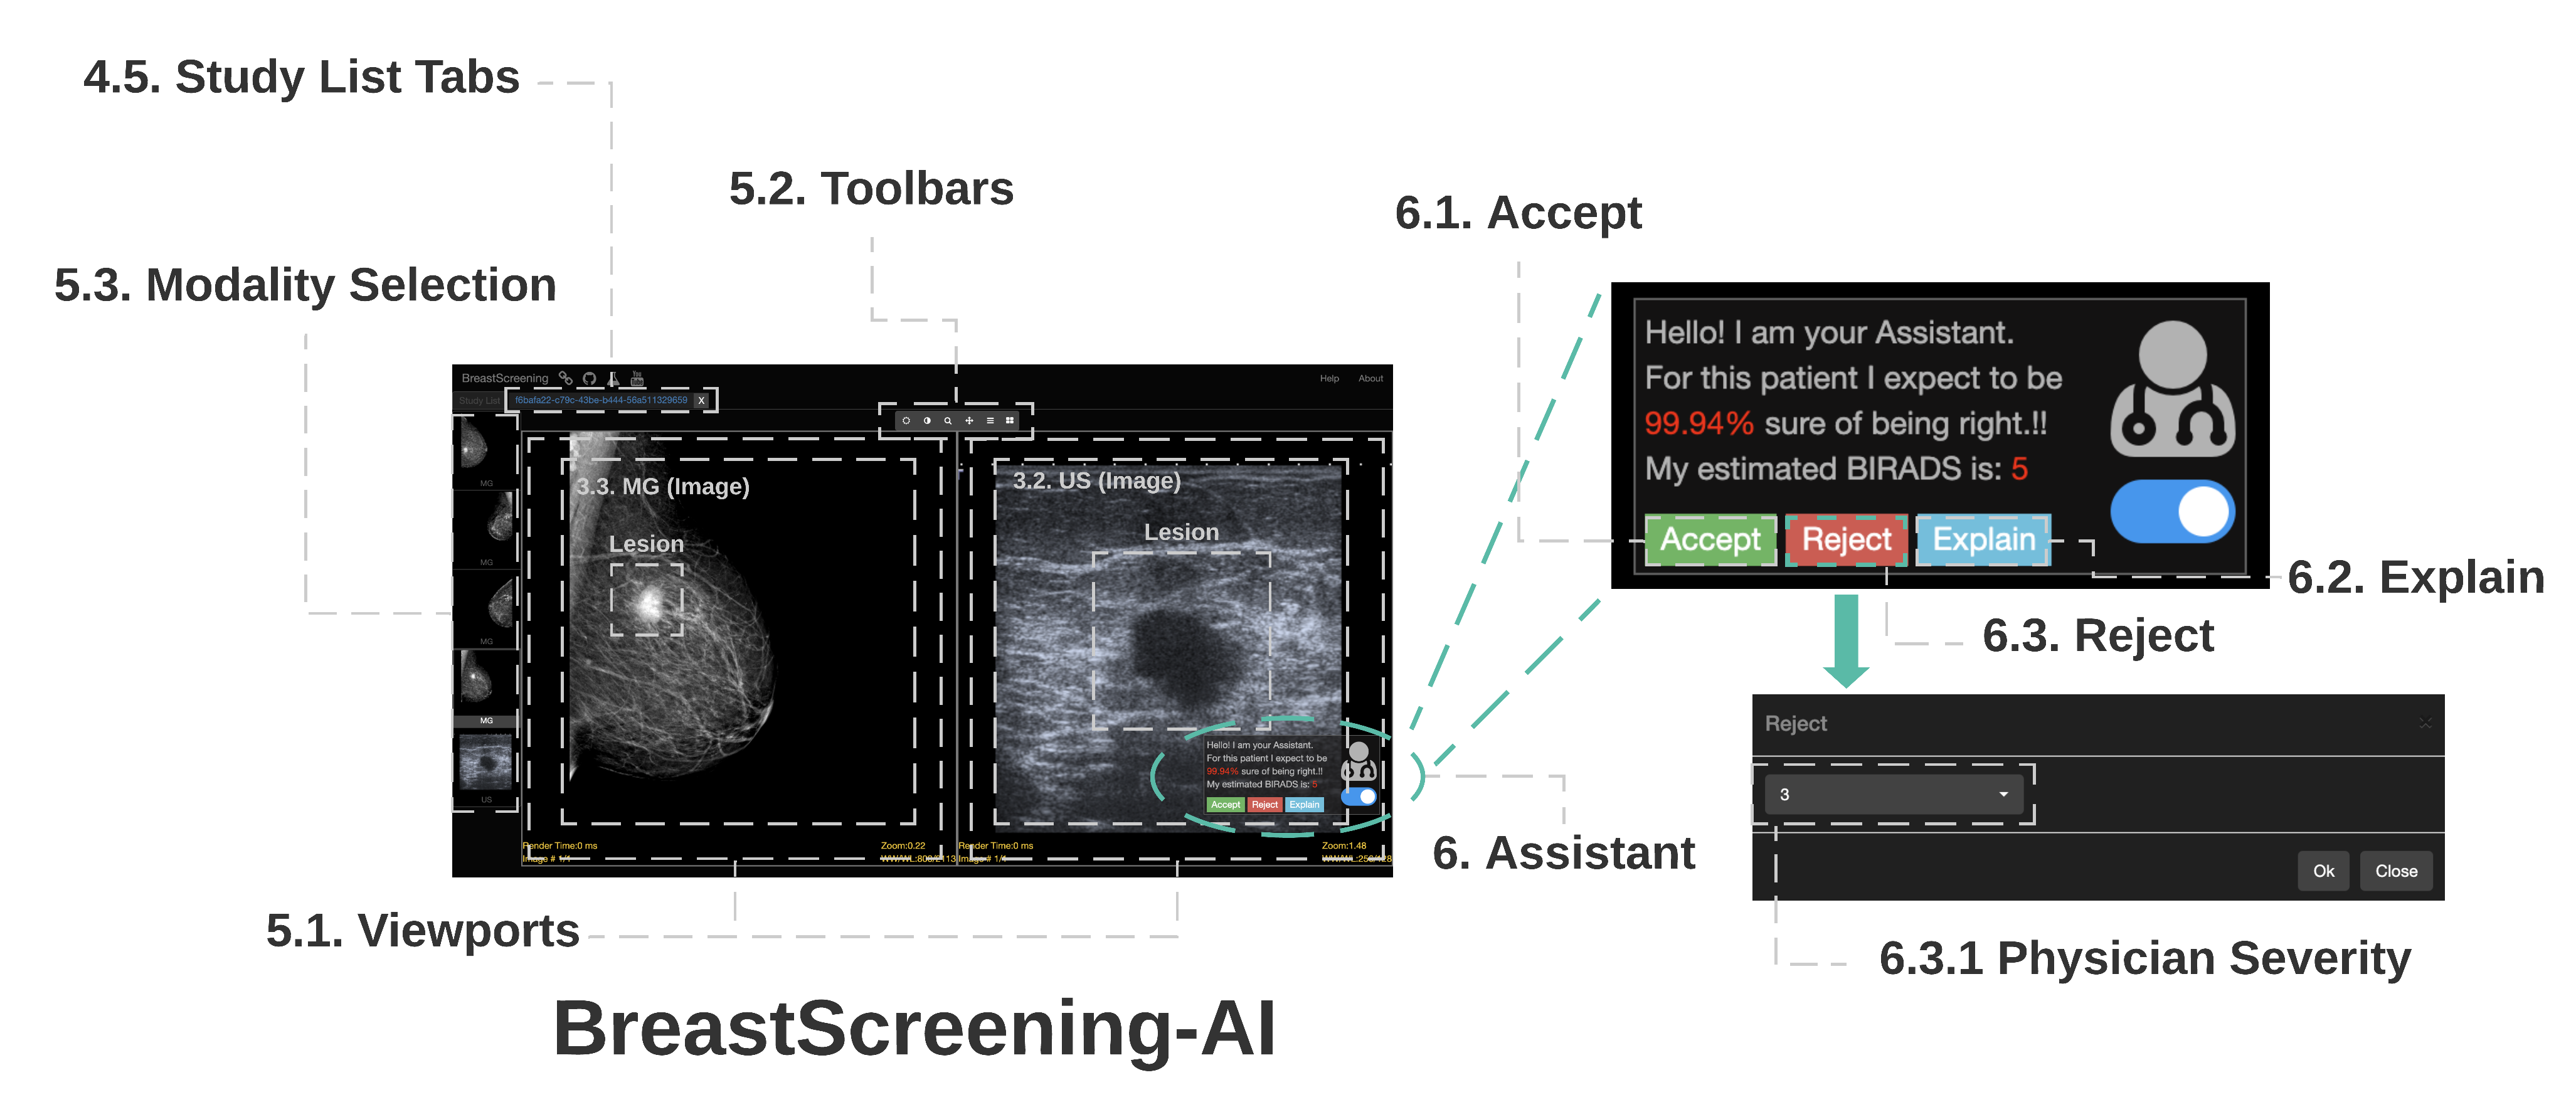
\includegraphics[width=\textwidth]{images/fig031}
\caption{The {\it BreastScreening-AI} prototype provides several functionalities regarding the basics of {\it radiomics}. From there, clinicians are able to validate the integrated DenseNet classifier for the BI-RADS value.}
\label{fig:fig031}
\end{figure}
%%%%%%%%%%%%%%%%%%%%%%%%%%%%%%%%%%%%%%%%%%%%%%%%%%%

To summarize, the {\it BreastScreening} framework (Section~\ref{sec:sec004004001001}) is used by default for image interpretation and labelling on breast cancer diagnosis.
Due to the integration of intelligent agents, the new developments of the {\it BreastScreening-AI} prototype were giving this thesis the opportunity to test properly what are the implications of \ac{AI} techniques on the \ac{RRR} workflow.
Such implications are achieved through the implementation and integration of a classifier model (DenseNet) into the designed \ac{UI}.
By showing the work design decisions, the following sections will cover these prototyping directions.

\subsection{User Interface}
\label{sec:sec005004002}

Based on identified user needs (Section~\ref{sec:sec002005} and Section~\ref{sec:sec005003003}), the \ac{UI} was designed and implemented.
This \ac{UI} includes a set of refinement mechanisms to guide clinicians during the diagnostic process.
The \ac{UI} of {\it BreastScreening-AI} consists of two main components, comprising the list of patients (Figure~\ref{fig:fig003}) and medical imaging views (Figure~\ref{fig:fig031}).

The first assistant view is the {\it 4. List of Patients Views}.
With this view, clinicians can quickly choose the respective {\it 4.1. List of Patients}.
Using the \ac{BI-RADS} functionality ({\it 6.3.1.~Physician Severity}), clinicians can now classify (Figure~\ref{fig:fig031}) the severity of the breast lesion for each patient.
This {\it 4.1. List of Patients} contains only the most important and required information, avoiding the excess of data ({\it e.g.}, gender, access activity on the file, etc), typically shown on these systems.
Therefore, improving the medical imaging (\ac{MID}) visualization (Section~\ref{sec:sec005003002}) across the \ac{RRR} (Section~\ref{sec:sec002005}).
The {\it 4.5. Study List Tabs} also allows clinicians to switch between diagnosed patients, {\it 5. Medical Imaging Diagnosis Views}, and {\it 4. List of Patients Views}.

Upon starting the \ac{UI} in the web browser, the user can select from the {\it 4.1. List of Patients} available in the study list.
Hence, it will improve the design around medical imaging (\ac{MID}) at a higher diagnostic accuracy level (Section~\ref{sec:sec005006001006}) for a single clinician.
From here, users can search all patients using criteria such as {\bf Patient ID}, {\bf Study Date}, available {\bf Modality} sets, {\bf Study Description}, and number of {\bf Images}.
By pressing in a selected row, clinicians open the image viewers.
In the image viewers, it is possible to visualize the image modalities.

To support clinicians, {\it 4.3. Help} and {\it 4.4. About} components were provided.
The components are providing clinicians information about how to classify and information about the system, such as how to proceed in a specific use case.
For instance, these components mainly were used by Interns, to better understand how they could use the tool for diagnosis.
The {\it 5.2. Toolbars} (Figure \ref{fig:fig031}) were positioned to match the user's requirements (conclusions drawn during observations and interviews).
This corresponds to the MID goal (Section~\ref{sec:sec005003002}).
The {\it 5.1. Viewports} are displayed at the right, after the {\it 5.2. Toolbars}.

Clinicians can probe for lesion patterns via the {\it 5.1.~Viewports}.
From here, clinicians can process the image by using the {\it 5.2.~Toolbars} features ({\it MID}).
Each time the {\it 5.2.~Toolbars} functionalities are activated, the clinician needs to perform a simple and easy interaction with the medical image to manipulate it as desired.
Using the {\it 5.2.~Toolbars} on the {\it 5.1.~Viewports}, the clinician can locate the lesions and classify its severity (\ac{BI-RADS}).

In this section, the document describe the minor set of designed functionalities of the \ac{UI}.
Some of these functionalities are already mapped to the respective design goal (Section~\ref{sec:sec005003002}).
However, some functionalities were not yet mapped.
The following sections will map the two main \ac{UI} functionalities, {\it i.e.}, assistant (Section~\ref{sec:sec005004002001}) and explainability (Section~\ref{sec:sec005004002002}), with the design goals (Section~\ref{sec:sec005003002}).

\subsubsection{Assistant}
\label{sec:sec005004002001}

The {\it 6.1.~Accept} or {\it 6.3.~Reject} allows the clinician to accept (or reject) the automatic classification of the {\it 6.~Assistant}.
The {\it 6.~Assistant} is based on the use of a DenseNet~\cite{Huang_2017_CVPR}.
However, integrating a \ac{DNN} needs special attention.
Typically, the training of a \ac{DNN} is expensive regarding the time spent, since its classification performance will improve as the training dataset becomes larger.
Thus, training the model from scratch is not the best option.
For this reason, we pre-train ({\it i.e.} off-line training before the \ac{UI} integration) the \ac{DNN} on ImageNet~\cite{10.1145/3351095.3375709} dataset and fine-tuned using our multi-modal breast dataset.
Specifically, we fine-tune the \ac{DNN} using supervised learning.
Only afterwards, the pre-trained DenseNet is incorporated into the \ac{UI}.

The implemented DenseNet takes medical images as an input and outputs the severity probability.
The input consists of images ({\it i.e.} \ac{MG}, \ac{US} and \ac{MRI} slices) with the corresponding label ({\it i.e.}, the \ac{BI-RADS}) that is previously classified by an expert.
The output consists of having five nodes in the last layer of the \ac{DNN}.
Each node is assigned to a given class that corresponds to each \ac{BI-RADS} score.
After this stage, we have conditions for the integration, since now the DenseNet is tuned to perform the classification in unseen test images.
The classification is fast, being tailored for an online diagnosis.

When several modalities (\ac{MID} and \ac{CRD}) are correctly used (regarding the {\it 5.3.~Modality~Selection} on a multimodality view), the clinician can find more accurately the right severity classification, as concluded in Section~\ref{sec:sec005006001006}.
For the {\it 6.3.~Reject} option, the physician will have the opportunity to insert (\ac{CRD}) the proposed BIRADS on a drag-and-drop menu ({\it 6.3.1.~Physician Severity}) of severity options. Both \ac{MID} and \ac{CRD} goals are supporting our {\bf RQ5.1} question (Section~\ref{sec:sec005001002}).

\subsubsection{Explainability}
\label{sec:sec005004002002}

Finally, the clinician may press for the {\it 6.2.~Explain} functionality  by looking at the generated heatmaps (Figure~\ref{fig:fig032}).
The generation of the above colour maps come from the following information: (i) the area ({\it Lesion Size}) of the lesion that comes from the delineation process, (ii) the circularity/sharpness ({\it Lesion Shape}) that can be computed from the annotation in (i), and (iii) the BI-RADS score automatically provided by the DenseNet ({\it i.e.}, classifier intelligent agent).
The \ac{ED} design goal is performed as above described helping to answer to research questions {\bf RQ5.2} and {\bf RQ5.3} (Section~\ref{sec:sec005001002}).

Covered by the \ac{ED} design goal, the thesis can provide a key component (Section~\ref{sec:sec003006}) to disambiguate the \ac{AI} result with the application of an explanation technique.
For a better prediction, the result of this explanation process is a heatmap visualizing the importance of each pixel.
With heatmaps, clinicians can capture and understand the logic arguments of the DenseNet (Section~\ref{sec:sec005006002}) by giving images and pixels a colour meaning of the lesion severity.
Thus, the \ac{ED} design goal is bringing the opportunity to disambiguate this \ac{DL} method for more transparent and explainable (\ac{XAI}) process.
Next, the section will describe the applied study methods to prove these claims.


%%%%%%%%%%%%%%%%%%%%%%%%%%%%%%%%%%%%%%%%%%%%%%%%%%%
\begin{figure}[htbp]
\centering
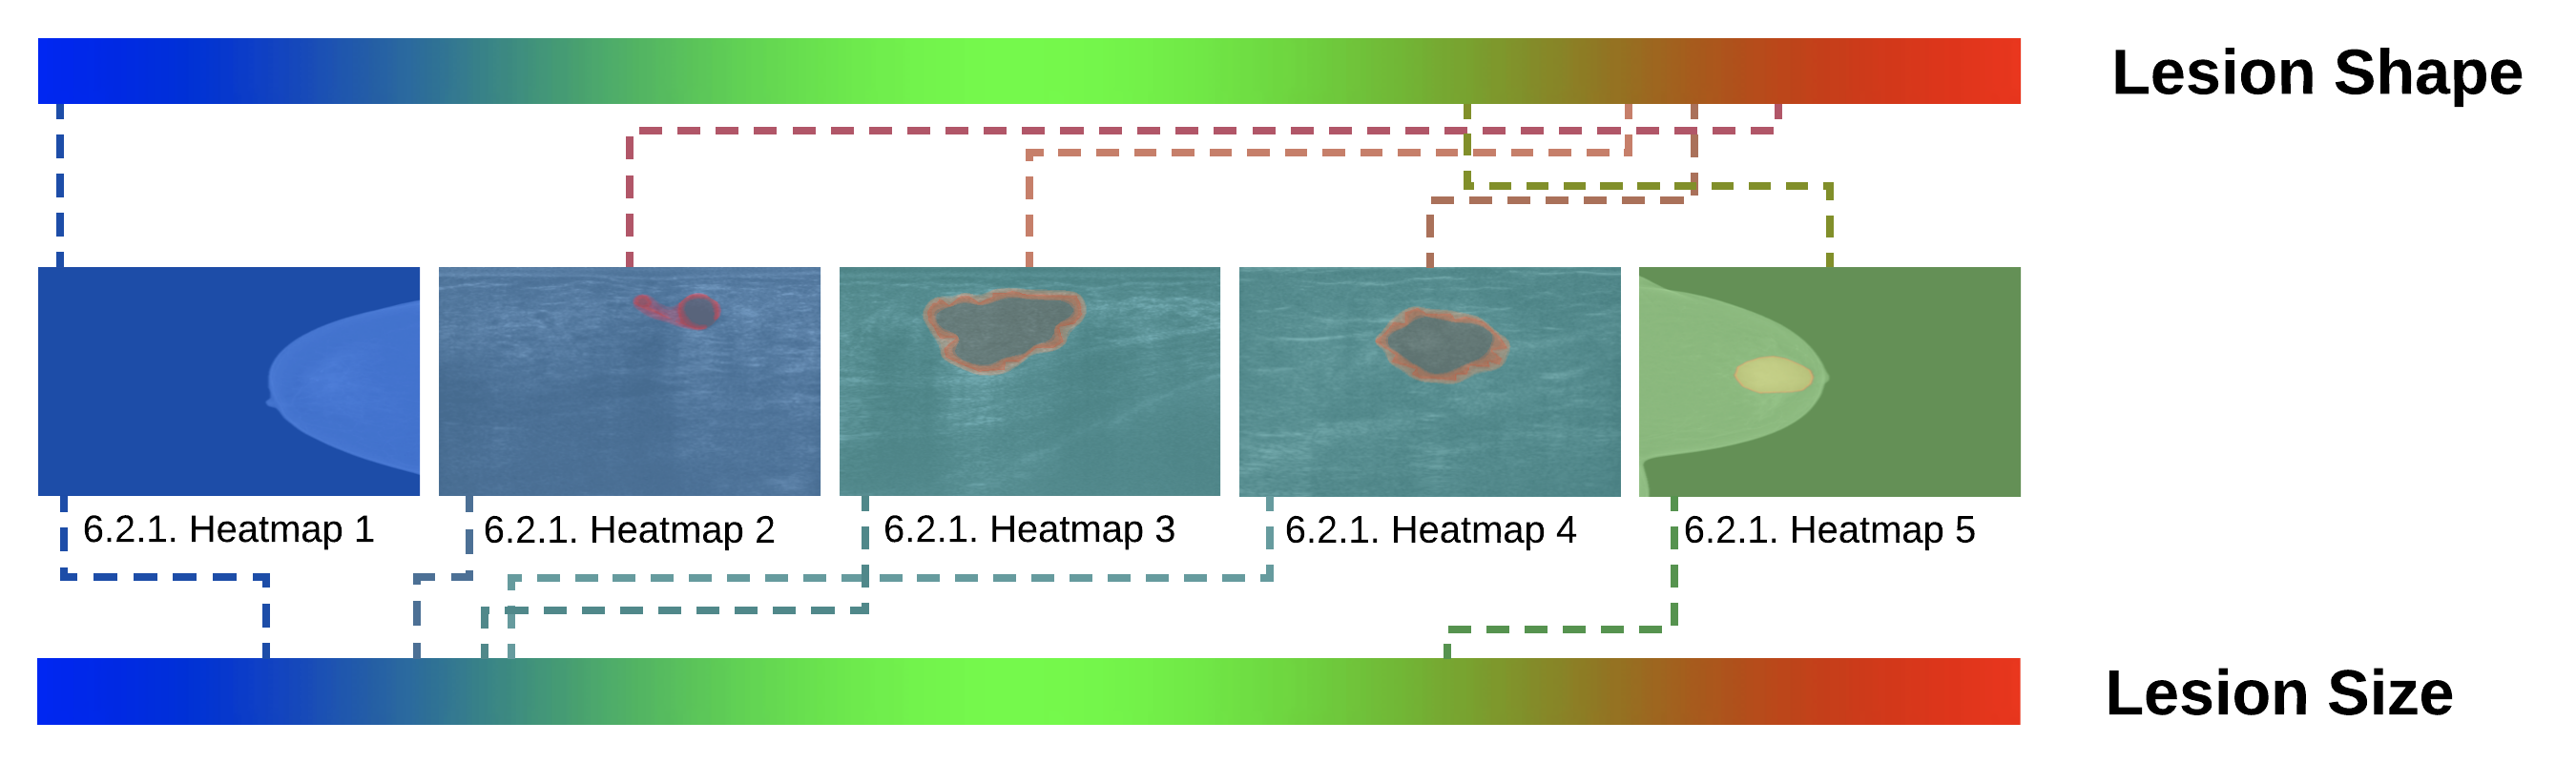
\includegraphics[width=\columnwidth]{images/fig032}
\caption{On {\it 6.2.~Explain}, the assistant will pop-up several {\it heatmaps}. The {\it heatmaps} represent two different scales: (a) {\it Shape}; and (b) {\it Size} of the lesion. First, the model computes the BI-RADS using the DenseNet classification. Second, the model computes the lesion circularity (top scale) and size (bottom scale) and associate it to the colors regarding both circularity/size and BI-RADS.}
\label{fig:fig032}
\end{figure}
%%%%%%%%%%%%%%%%%%%%%%%%%%%%%%%%%%%%%%%%%%%%%%%%%%%

\section{Methods}
\label{sec:sec005005}

For this study, an evaluation of {\it BreastScreening-AI} simulating real world conditions with 45 clinicians in nine different clinical institutions was conducted.
The study goal was to quantitatively (Section~\ref{sec:sec005006001}) and qualitatively (Section~\ref{sec:sec005006002}) assess the proposed design principles that the {\it BreastScreening-AI} embodies and to understand how these principles would work in practice.
The experimental setup aimed at testing two conditions: {\bf Cond. C1} - {\it Current}, {\it i.e.}, a multimodality strategy without any \ac{AI}-assisted technique; {\bf Cond. C2} - multimodality strategy taking advantage of the  \ac{AI}-assisted ({\it e.g.}, DenseNet~\cite{9098470}), supporting clinician's second opinion and autonomous patient diagnostic.

\hfill

\noindent
For each condition, three classes of patients were defined:

%%%%%%%%%%%%%%%%%%%%%%%%%%%%%%%%%%%%%%%%%%%%%%%%%%%
\begin{itemize}
\item {\bf Class 1}: patients such that \ac{BI-RADS} $\leq$ 1 (low severity);
\item {\bf Class 2}: patients such that 1 $<$ \ac{BI-RADS} $\leq$ 3 (medium severity);
\item {\bf Class 3}: patients such that \ac{BI-RADS} $>$ 3 (high severity);
\end{itemize}
%%%%%%%%%%%%%%%%%%%%%%%%%%%%%%%%%%%%%%%%%%%%%%%%%%%

Having data available is challenging and requires multiple steps, including anonymization of data (Section~\ref{sec:sec004004001001}).
The ideal approach is collaboration between clinicians and \ac{AI} researchers, either in-house or through collaborative research agreements.
Therefore, a protocol was celebrated with Hospital Fernando Fonseca so that the interchange of patients could be possible.
The purpose of this protocol is to establish bases of collaboration in all scientific and technological areas, as well as education and training in which \ac{IST} and Hospital Fernando Fonseca carry out their activities.
From this protocol, the exams were annotated by eight radiologists and classified with a \ac{BI-RADS} severity from an expert doctor.
The expert doctor is the head of the radiologist services of Hospital Fernando Fonseca.

\subsection{Participants}
\label{sec:sec005005001}

In this study, participants were asked to practice with three predefined patients selected from the three above classes.
To accomplish this, each patient was randomly selected ({\it i.e.}, {\bf P1}, {\bf P2} and {\bf P3}) from each class ({\it i.e.}, {\bf Class 1}, {\bf Class 2} and {\bf Class 3}), respectively.
Then, participants were asked to diagnose each patient.
A natural expectation is that the intelligent agent would minimize the time required and accuracy ({\it e.g.}, improving \ac{FP} or \ac{FN} values).
The study involved 45 clinicians, recruited on a volunteer basis from a broad range of clinical scenarios, including nine different health institutions (two public hospitals, two cancer institutes and two private clinics).

\hfill

\noindent
In the following list, the number of clinicians and respective clinical institutions is provided:

\begin{multicols}{2}
\begin{itemize}
\item 12 clinicians of Hospital Fernando Fonseca; % HFF
\item 10 clinicians of IPO Lisboa; %IPOL
\item 2 clinicians of Hospital Santa Maria; %HSM
\item 9 clinicians of IPO Coimbra; %IPOC
\item 1 clinician of Madeira Medical Center; and %MMC
\item 1 clinician of Hospital SAMS; %SAMS
\item 8 clinicians of Hospital do Barreiro; %HB
\item 1 clinician of Hospital Santo Ant\'{o}nio; %HSA
\item 1 clinician of Jo\~{a}o Carlos Costa Clinic. %JCC
\end{itemize}
\end{multicols}

Before the experiment, clinicians first filled out a pre-study questionnaire eliciting demographic information (Appendix~\ref{chap:appendix}), including age group, gender, medical professional experience, between others.
From the demographic questionnaires:
24.4\% of the clinicians have between 31 and 40 years of practical experience (seniors);
31.1\% have between 11 and 30 years of experience (middles);
17.8\% have between 6 and 10 years of experience (juniors); and
26.7\% have limited experience (interns).
Interviews were conducted in a semi-structured fashion taking about 30 minutes.
Overall, 57 days were spent on the clinical institutions for the observation process and six months for the classification.

\subsection{Procedure}
\label{sec:sec005005002}

After providing informed consent for participation in the study, clinicians reported information about their demographics (age, gender, etc) and professional background (professional or academic training, number of years of clinical experience).
Next, clinicians familiarized themselves for about 30 seconds with \ac{UI} and with the basic interface components common to both {\bf Cond. C1} and {\bf Cond. C2} conditions (Section~\ref{sec:sec005005}).
However, the two conditions are different.

The first condition ({\bf Cond. C1}) relies on classifying patients without \ac{AI} assistance~\cite{10.1145/3399715.3399744}.
The goal was to understand what is the actual clinicians' performance.
Thus, a simulation of the current clinicians' available tools on the \ac{RRR} was held, while interacting with the first developed tool (Figure~\ref{fig:fig028}).

For the second condition ({\bf Cond. C2}), the procedure required to reject (or accept) the proposed \ac{BI-RADS} provided by the intelligent agent~\cite{https://doi.org/10.13140/rg.2.2.16566.14403/1}.
At this stage, participants will interact with the new prototype ({\it i.e.}, {\it BreastScreening-AI}) using the multi-modal dataset acquired and curated under this thesis.
Actually, this work has a total of 415 patient cases.
In the dataset, there exists cases where the patient does not have all the image modalities (recall Figure~\ref{fig:fig018} where the acquisition may finish before all the modalities are available).
Thus, the following requirements were defined to conduct the study work analysis.

\hfill

\noindent
The requirements are as follows:

%%%%%%%%%%%%%%%%%%%%%%%%%%%%%%%%%%%%%%%%%%%%%%%%%%%
\begin{enumerate}
\item All patients must have each of the three available modalities;
\item All patients were annotated and classified by radiologists team of Hospital Fernando Fonseca;
\item The patients were grouped in low, medium and high severity according to the \ac{BI-RADS};
\end{enumerate}
%%%%%%%%%%%%%%%%%%%%%%%%%%%%%%%%%%%%%%%%%%%%%%%%%%%

The above procedure allowed this work to obtain a set of 415 cases.
Notice that the dataset is partitioned according to the three classes above mentioned.
Similar for both conditions ({\bf Cond. C1} and {\bf Cond. C2}), the first task was to fill pre-test forms, as already mentioned.
The second task was the user characterization form, providing demographic data about participants.
Next, each participant accessed the system via a web browser.
Each of the 45 clinicians were assigned three patients ({\it e.g.}, {\bf P1}, {\bf P2} or {\bf P3}), for diagnosis.
Thus, for each clinician it was assigned one patient with low severity, one with medium severity and another one with high severity.

When analysing the patients, for the second condition ({\bf Cond. C2}), the main task was to {\it accept} or {\it reject} the proposed \ac{BI-RADS} value provided by an intelligent agent.
In case of {\it rejecting} the proposed value, participants were asked to provide a new \ac{BI-RADS} value on the \ac{UI}.
An {\it explain} functionality was provided to be used informing participants concerning where and how much sever the lesions are (Figure~\ref{fig:fig032}).
However, for the first condition ({\bf Cond. C1}), the \ac{BI-RADS} classification was provided by clinicians in the end of patient analysis alongside filling a form~\cite{https://doi.org/10.13140/rg.2.2.36306.86725}.
These setups will be used to support the work results (Section~\ref{sec:sec005006}).

Before the main test, every interaction was shown by the facilitator and upcoming questions were clarified.
In the end, for each participant it was applied both \ac{SUS}~\cite{Tyllinen:2016:WNN:2858036.2858570} and \ac{NASA-TLX}~\cite{ramkumar2017using, grier2015high} on two different questionnaires~\cite{https://doi.org/10.13140/rg.2.2.25301.06883, https://doi.org/10.13140/rg.2.2.26978.79044} for usability\footnotemark[21] and workload\footnotemark[22] measurements.
Finally, a {\it post-task} questionnaire~\cite{https://doi.org/10.13140/rg.2.2.16566.14403/1} was carried out.

%%%%%%%%%%%%%%%%%%%%%%%%%%%%%%%%%%%%%%%%%%%%%%%%%%%
\footnotetext[21]{For SUS scores, we used a 5 item scale. The scores range from 1 - "{\bf Strong Disagree}" to 5 - "{\bf Strong Agree}". The mean across all individual questionnaires was computed over studies. We provide an available {\it dataset} (\href{https://mimbcd-ui.github.io/dataset-uta7-sus/}{mimbcd-ui.github.io/dataset-uta7-sus}) from our SUS data.}
%%%%%%%%%%%%%%%%%%%%%%%%%%%%%%%%%%%%%%%%%%%%%%%%%%%

%%%%%%%%%%%%%%%%%%%%%%%%%%%%%%%%%%%%%%%%%%%%%%%%%%%
\footnotetext[22]{For NASA-TLX scores, we used a 20 item scale. The scores range from 1 - "{\bf Very Low}" to 20 - "{\bf Very High}". Again, we provide an available {\it dataset} (\href{https://mimbcd-ui.github.io/dataset-uta7-nasa-tlx/}{mimbcd-ui.github.io/dataset-uta7-nasa-tlx}) from our NASA-TLX data.}
%%%%%%%%%%%%%%%%%%%%%%%%%%%%%%%%%%%%%%%%%%%%%%%%%%%

\subsection{Analysis}
\label{sec:sec005005003}

The study of {\it BreastScreening-AI} included both quantitative (Section~\ref{sec:sec005006001}) and qualitative (Section~\ref{sec:sec005006002}) analysis.
For the qualitative analysis\footnotemark[23], user interactions were tracked across the prototype using \href{https://www.hotjar.com/}{Hotjar}~\cite{liikkanen2017data}.
To record the task activities and the interview, screen and sound recordings were resorted.
Finally, \href{https://www.tobiipro.com/product-listing/tobii-pro-sdk/}{Tobii Pro SDK}~\cite{chatelain2018evaluation} was used for eye tracking and gaze information.
For the quantitative analysis\footnotemark[24] the well known \ac{SUS}~\cite{Tyllinen:2016:WNN:2858036.2858570} was used to objectively measure the usability\footnotemark[25] of the intelligent agent setup to answer {\bf RQ5.3}.

To measure the effectiveness performance of the intelligent agent introduction, the \ac{NASA-TLX}~\cite{ramkumar2017using, grier2015high} was used, assessing the perceived workload\footnotemark[26] to answer {\bf RQ5.1}.
The diagnostic classification was also measured to find correlations with the breast severity.
Finally, the number of \acp{FP} and \acp{FN} were measured to understand severity rates.

%%%%%%%%%%%%%%%%%%%%%%%%%%%%%%%%%%%%%%%%%%%%%%%%%%%
\footnotetext[23]{By {\bf qualitative analysis}, it means the observational findings from clinicians that identify and answer our design methods and features to use. The {\bf qualitative data} was divided into two groups: (1) {\bf qualitative attitudinal data}; and (2) {\bf qualitative behavioral data}. The first one, can be defined as clinician's thoughts, beliefs and self-reported needs obtained from the user interviews, focus groups and affinity diagrams.}
%%%%%%%%%%%%%%%%%%%%%%%%%%%%%%%%%%%%%%%%%%%%%%%%%%%

%%%%%%%%%%%%%%%%%%%%%%%%%%%%%%%%%%%%%%%%%%%%%%%%%%%
\footnotetext[24]{By {\bf quantitative analysis}, it means the use of metrics to measure tasks, which will reflect on the task performance, efficiency and efficacy. Measuring {\bf quantitative data} offer an indirect assessment of the design usability as well.}
%%%%%%%%%%%%%%%%%%%%%%%%%%%%%%%%%%%%%%%%%%%%%%%%%%%

%%%%%%%%%%%%%%%%%%%%%%%%%%%%%%%%%%%%%%%%%%%%%%%%%%%
\footnotetext[25]{Regarding {\bf SUS} scores, clinicians were provided with an individual questionnaire on a scale that is easily understood. We used {\bf SUS} to measure the intelligent agent usability. The scale provides helpful information about a clinician's takeaways and overall experience during diagnostic.}
%%%%%%%%%%%%%%%%%%%%%%%%%%%%%%%%%%%%%%%%%%%%%%%%%%%

%%%%%%%%%%%%%%%%%%%%%%%%%%%%%%%%%%%%%%%%%%%%%%%%%%%
\footnotetext[26]{The {\bf NASA-TLX} scale was used to measure the perceived workload required by the complex, highly demanding tasks of medical imaging diagnosis on the radiology room.}
%%%%%%%%%%%%%%%%%%%%%%%%%%%%%%%%%%%%%%%%%%%%%%%%%%%

Although \ac{SUS} is more regularly used as single score, in this study the scale was used as individual questionnaires.
Individual \ac{SUS} scores have typically negative skew~\cite{lewis2018system}, but the the mean sample values are usually normal distributed.
Therefore, taking advantage of this statistical behaviour to compute the quantitative analysis (Section~\ref{sec:sec005006001}) was held under this thesis.
On the other hand, the basic \ac{NASA-TLX} scores were used, which are highly reliable~\cite{ramkumar2017using}.
\ac{NASA-TLX} questionnaire consistently exhibits high reliability, user acceptance and low inter-subject variability to measure workload.
In this study, \ac{NASA-TLX} was used to identify clinicians' workload during various stages of the workflow.
Clinicians were asked to complete both \ac{SUS} and \ac{NASA-TLX} scores.

In the end of the three patients' diagnostics, a {\it post-task} questionnaire was performed.
Rating the intelligent agent experience and performance during the diagnostic time period, was the goal with those questionnaires.
The above measurements are part of the quantitative analysis with a comparison between {\it Current} ({\bf Cond. C1}) and \ac{AI}-assisted ({\bf Cond. C2}) setups.
With this comparison, it will answer both {\bf RQ5.1} and {\bf RQ5.2} providing evidence for the impact and expectations of \ac{AI} assistance on the \ac{RRR} workflow.
For the qualitative analysis, opinion-based feedback was extracted from the recorded audio.
The received feedback was translated to a set of sentences counting the number of clinicians who had the same similar opinion.
Clinicians were asked to provide feedback concerning how they decided for each patient case ({\it i.e.}, {\bf P1}, {\bf P2} and {\bf P3}), what information they used to make these decisions, and how the explainability information affected their decision-making.
Recurring themes are reported below.

\section{Results}
\label{sec:sec005006}

In this section, several concerns will be studied by performing a set of quantitative and qualitative analysis of participants' information and behaviour.
As follows, the document will cover each one.

\subsection{Quantitative Analysis}
\label{sec:sec005006001}

In this study, the quantitative analysis takes into account differences between medical expert levels ({\it i.e.}, {\it Intern}, {\it Junior}, {\it Middle}, and {\it Senior}), user characteristics, and medical imaging interpretation to understand user behaviour during decision-making.
In this section, the goal is providing a general and straightforward approach to do a quantitative analysis and inference understanding on data collected during user studies.

The \ac{SUS} questionnaire was used within the context of assessing {\it BreastScreening-AI} usability.
Hereby, obtained results are described from the {\it \ac{SUS} Scores} and {\it \ac{SUS} Questions} (Figures \ref{fig:fig033}, \ref{fig:fig034}, \ref{fig:fig035} and \ref{fig:fig036}).
Subjective feedback of the interviews was provided from the number of participants who expressed a given comment.
By analyzing the numbers, a highly positive adoption was obtained from the {\it Assistant} condition (Figures \ref{fig:fig034} and \ref{fig:fig036}) in comparison to the {\it Current} condition (Figures \ref{fig:fig033} and \ref{fig:fig035}), as described next.

\hfill

\noindent
Hence, four relations emerged under this analysis:

%%%%%%%%%%%%%%%%%%%%%%%%%%%%%%%%%%%%%%%%%%%%%%%%%%%
\begin{enumerate}[label=\alph*]
\item - differences between {\it \ac{SUS} Scores} and {\it \ac{SUS} Questions} (Figures \ref{fig:fig033}, \ref{fig:fig034}, \ref{fig:fig035} and \ref{fig:fig036}) across the groups of medical experience ({\it i.e.}, {\it Intern}, {\it Junior}, {\it Middle}, and {\it Senior}) on the {\it Assistant} setup;
\item - workload measurements (Tables \ref{tab:tab001} and \ref{tab:tab002}) of both {\it Current} and {\it Assistant} setups;
\item - relation between diagnostic {\it Time} and lesion severity ({\it i.e.}, Low, Medium and High values of the BI-RADS) on both conditions ({\it i.e.}, {\it Current} and {\it Assistant}), among different groups of medical experience (Figure \ref{fig:fig037}); and
\item - False-Positive and False-Negative ratios (Figure \ref{fig:fig038});
\end{enumerate}
%%%%%%%%%%%%%%%%%%%%%%%%%%%%%%%%%%%%%%%%%%%%%%%%%%%

\subsubsection{{\it SUS Scores} vs {\it SUS Positive Questions}}
\label{sec:sec005006001001}

The generated results of the \ac{SUS} questionnaire are depicted in Figures \ref{fig:fig033} and \ref{fig:fig034}.
On the one hand, Figure ~\ref{fig:fig033} shows the results obtained with
{\it Current} scenario.
On the other hand, Figure~\ref{fig:fig034} shows the results with the introduction of the {\it Assistant}.
Both study conditions can be compared to understand usability improvements from the {\it Current} to {\it Assistant} scenario.
However, this claim will be further (Section~\ref{sec:sec005007}) discussed.
Next, the results are detailed.

%%%%%%%%%%%%%%%%%%%%%%%%%%%%%%%%%%%%%%%%%%%%%%%%%%%
\begin{figure}[htbp]
\centering
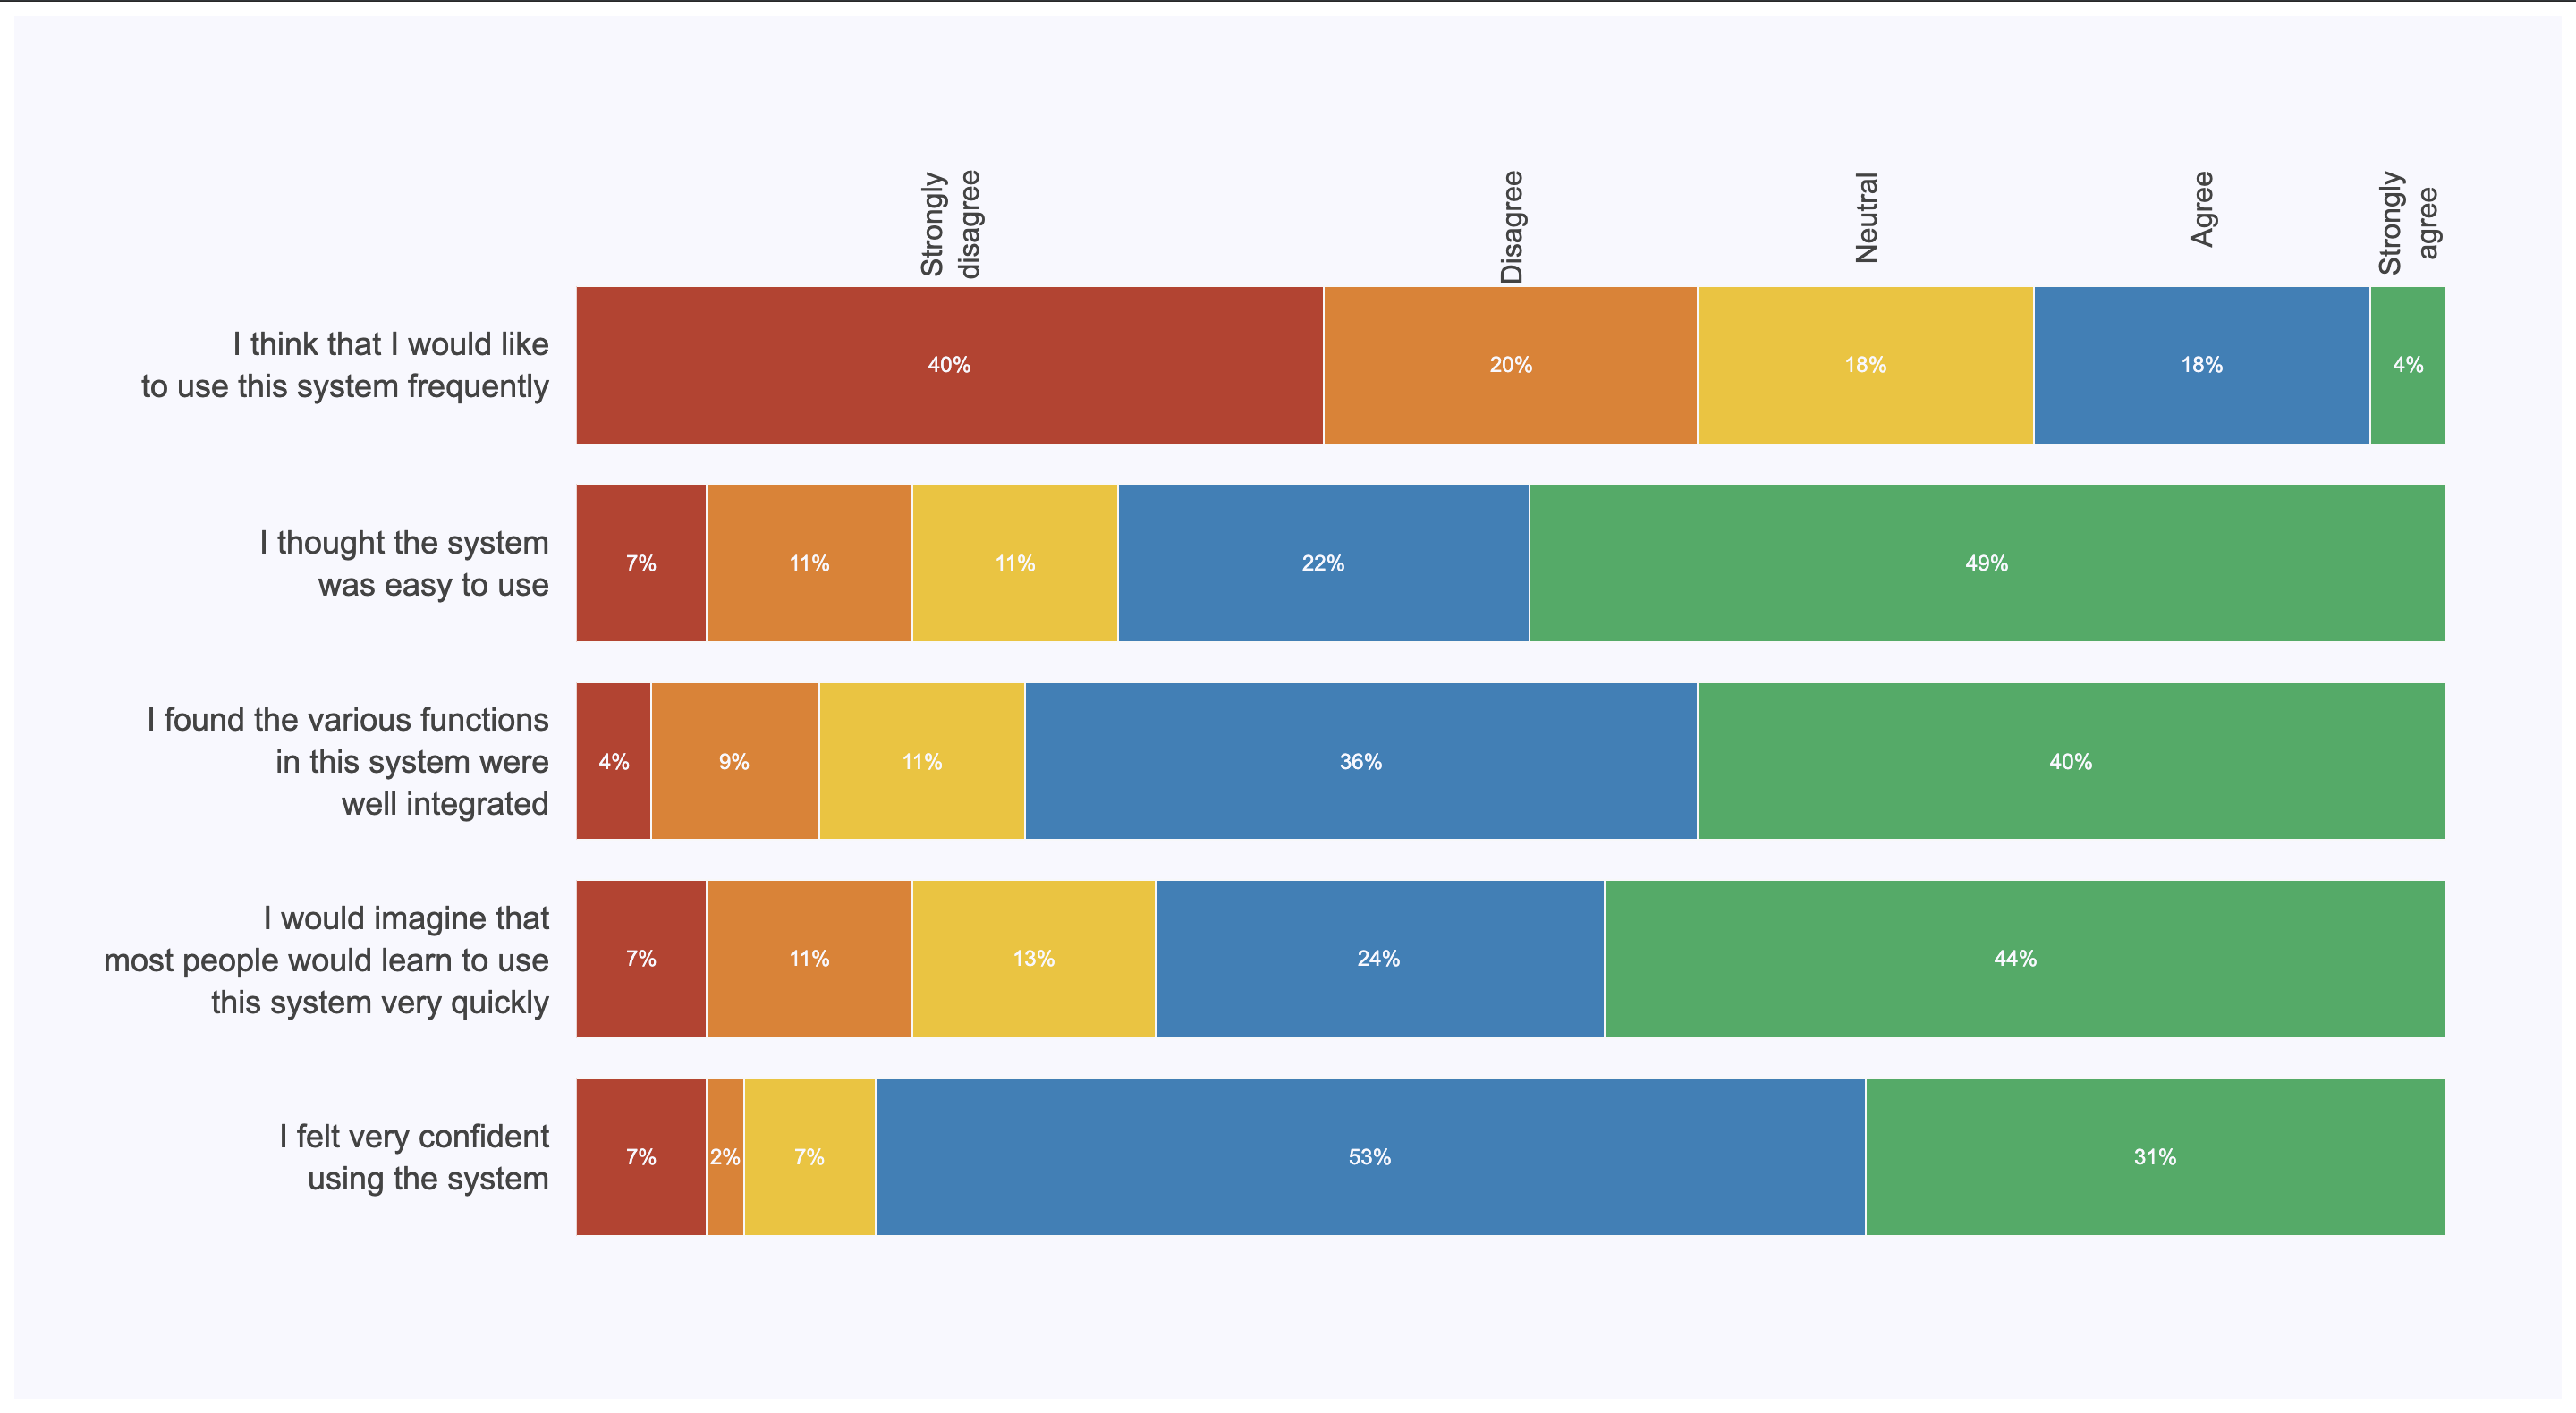
\includegraphics[width=\textwidth]{images/fig033}
\caption{Results of SUS with Positive Questions for the {\it Current} condition. Each color and respective bar number indicate the mean score for the question, {\it i.e.}, ranging from 1 = "Strongly disagree" to 5 = "Strongly agree". This figure represents the positive questions. The "Strongly agree" is the optimal value. From the reported results, a majority of the clinicians agree that the system was easy to use and with well integrated functionalities.}
\label{fig:fig033}
\end{figure}
%%%%%%%%%%%%%%%%%%%%%%%%%%%%%%%%%%%%%%%%%%%%%%%%%%%

%%%%%%%%%%%%%%%%%%%%%%%%%%%%%%%%%%%%%%%%%%%%%%%%%%%
\begin{figure}[htbp]
\centering
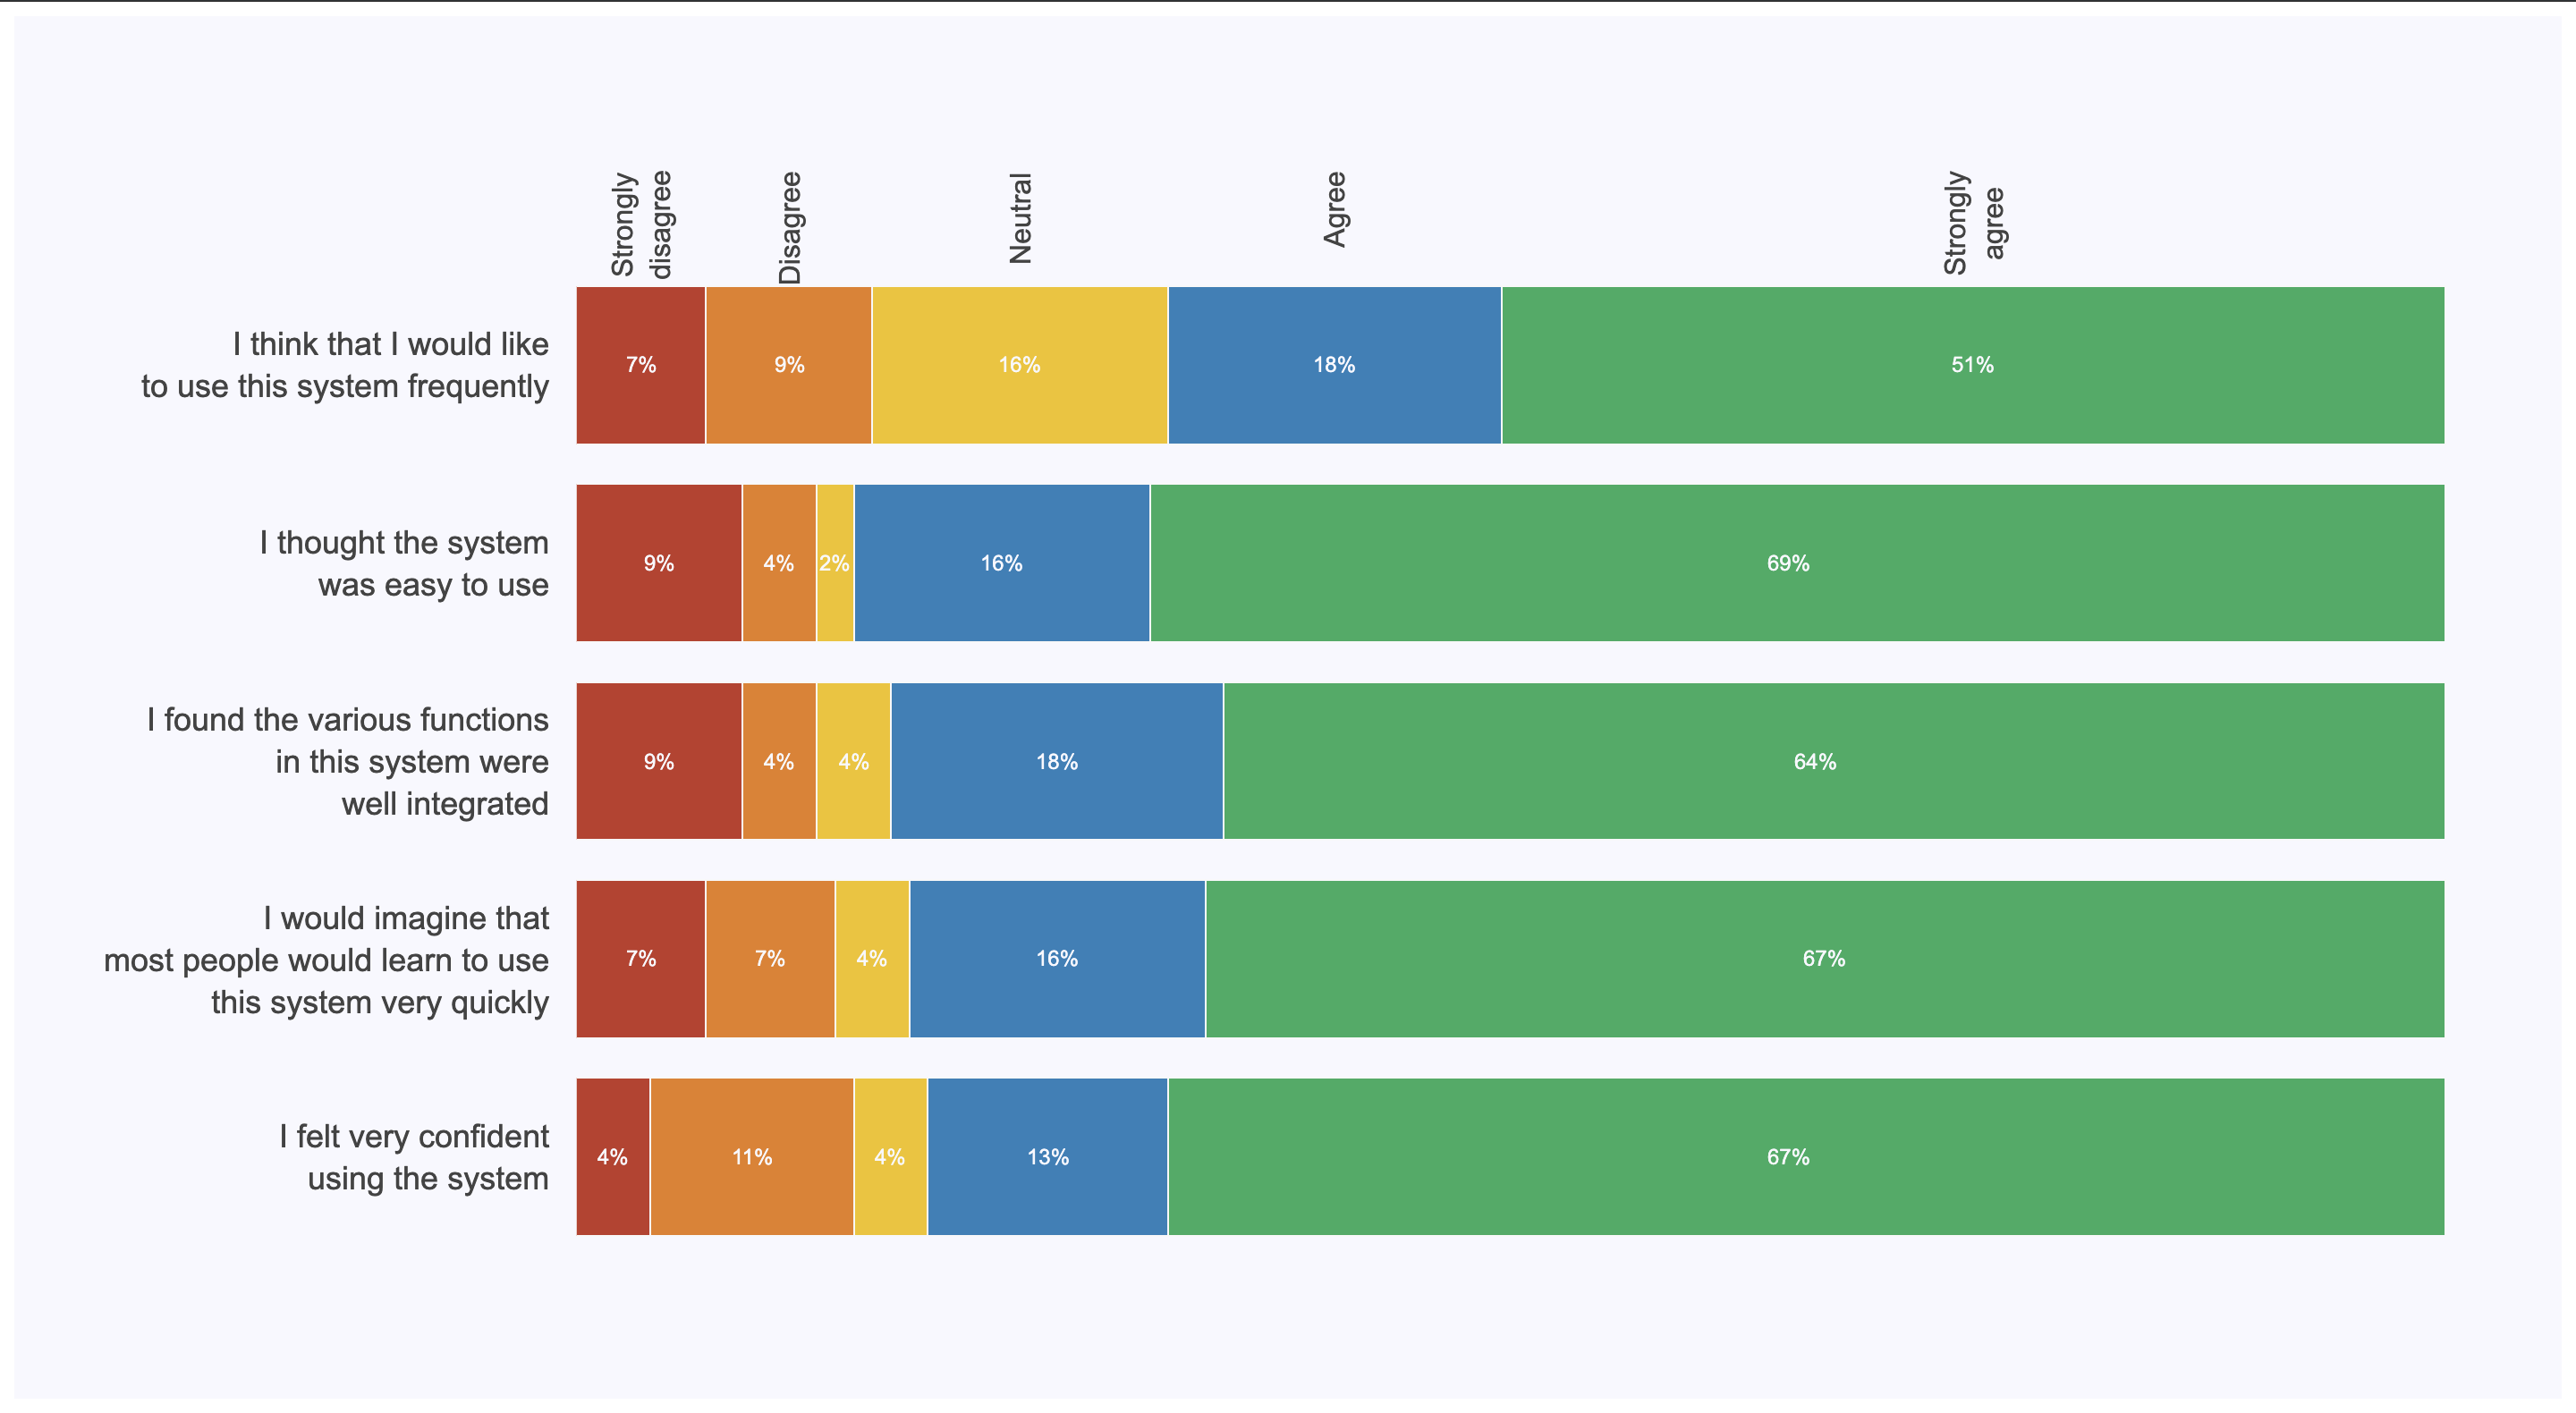
\includegraphics[width=\textwidth]{images/fig034}
\caption{Results of SUS with Positive Questions for the {\it Assistant} condition. This {\it Assistant} condition was well accepted by clinicians. Almost all clinicians would like to use this system frequently. Moreover, they consider the system much easier to use and with higher integrated functionalities. Last but not least, clinicians learn more quick and with more confidence this {\it Assistant} system condition.}
\label{fig:fig034}
\end{figure}
%%%%%%%%%%%%%%%%%%%%%%%%%%%%%%%%%%%%%%%%%%%%%%%%%%%

In short, the {\it Current} condition obtained 22\% of agreement against an obtained 69\% for the {\it Assistant} condition, revealing a higher acceptance for using the {\it Assistant} (Figure~\ref{fig:fig034}).
This means that despite of the clinicians' resistance of change for new tools~\cite{10.1145/3132272.3134111, gagnon2014electronic}, clinicians are now accepting this novel intelligent agents to support their clinical workflow.

Another clear fact to explain these values are the results for the easy of use.
In those results, the {\it Assistant} condition reveals an 85\% of agreement against the 71\% for the {\it Current} condition.
Conversely, 82\% of clinicians found that the various functions of the {\it Assistant} were well integrated with the workflow.
The confidence level with the {\it Assistant} condition was also very high, reaching 80\% on this condition.

Values of user confidence are also important to detail.
While using the {\it Current} condition, clinicians felt confident, where 53\% "Agree" and 31\% "Strongly agree" with this \ac{SUS} sentence.
A total of 84\% of agreement under the {\it Current} condition.
But more important, with the introduction of an intelligent agent this value was improved by far.
Although the total agreement value for the {\it Assistant} condition is inferior with 80\% in comparison to the {\it Current} condition, about 67\% of clinicians "Strongly agree" with the \ac{SUS} sentence.
Due to the high improvements of the "Strongly agree" sentence, it can be denoted that intelligent agents are increasing high values of confidence.
Such comparison will be further discussed (Section~\ref{sec:sec005007}) to clarify the achieved results.
Indeed, values of confidence will be extremely important to understand the impact for the introduction of \ac{AI} systems in the medical workflow, which will also be addressed with values of {\it trust} in Chapter~\ref{chap:chap006}.

\subsubsection{{\it SUS Scores} vs {\it SUS Negative Questions}}
\label{sec:sec005006001002}

Similarly to the previous analysis, here the same study was conducted, but now concerning the negative questions (Figure~\ref{fig:fig036}) of the scale.
Regarding the negative questions (Figure~\ref{fig:fig036}), 86\% of the clinicians disagree that the system is unnecessarily complex.
Suggesting that the introduction of an intelligent agent will not bring more complexity to the diagnostic.
Actually, these results are also paired with the \ac{NASA-TLX} (Tables \ref{tab:tab001} and \ref{tab:tab002}) results to prove this claim.

Concerning both {\it Current} and {\it Assistant} conditions, clinicians also answered two important \ac{SUS} statements addressing system inconsistency and cumbersome.
Specifically, about 44\% of clinicians "Strongly disagree" and 27\% "Disagree" for system inconsistency statement in the {\it Current} condition.
On the other hand, about 80\% of clinicians "Strongly disagree" and 4\% "Disagree" for system inconsistency statement in the {\it Assistant} condition.
Thus, by having a total of 84\% of disagreement, the {\it Assistant} condition was far improved, against the 71\% of the {\it Current} condition, with the introduction of an intelligent agent.
Moreover, in terms of the cumbersome \ac{SUS} statement, about 60\% "Strongly disagree" and 20\% "Disagree" that the {\it Current} condition was cumbersome.
For the {\it Assistant} condition, 80\% "Strongly disagree" and 4\% "Disagree" that the system is cumbersome.
A total of 84\% disagreement for cumbersome on the {\it Assistant} condition, which is more in comparison to the 80\% of the {\it Current} condition.

%%%%%%%%%%%%%%%%%%%%%%%%%%%%%%%%%%%%%%%%%%%%%%%%%%%
\begin{figure}[htbp]
\centering
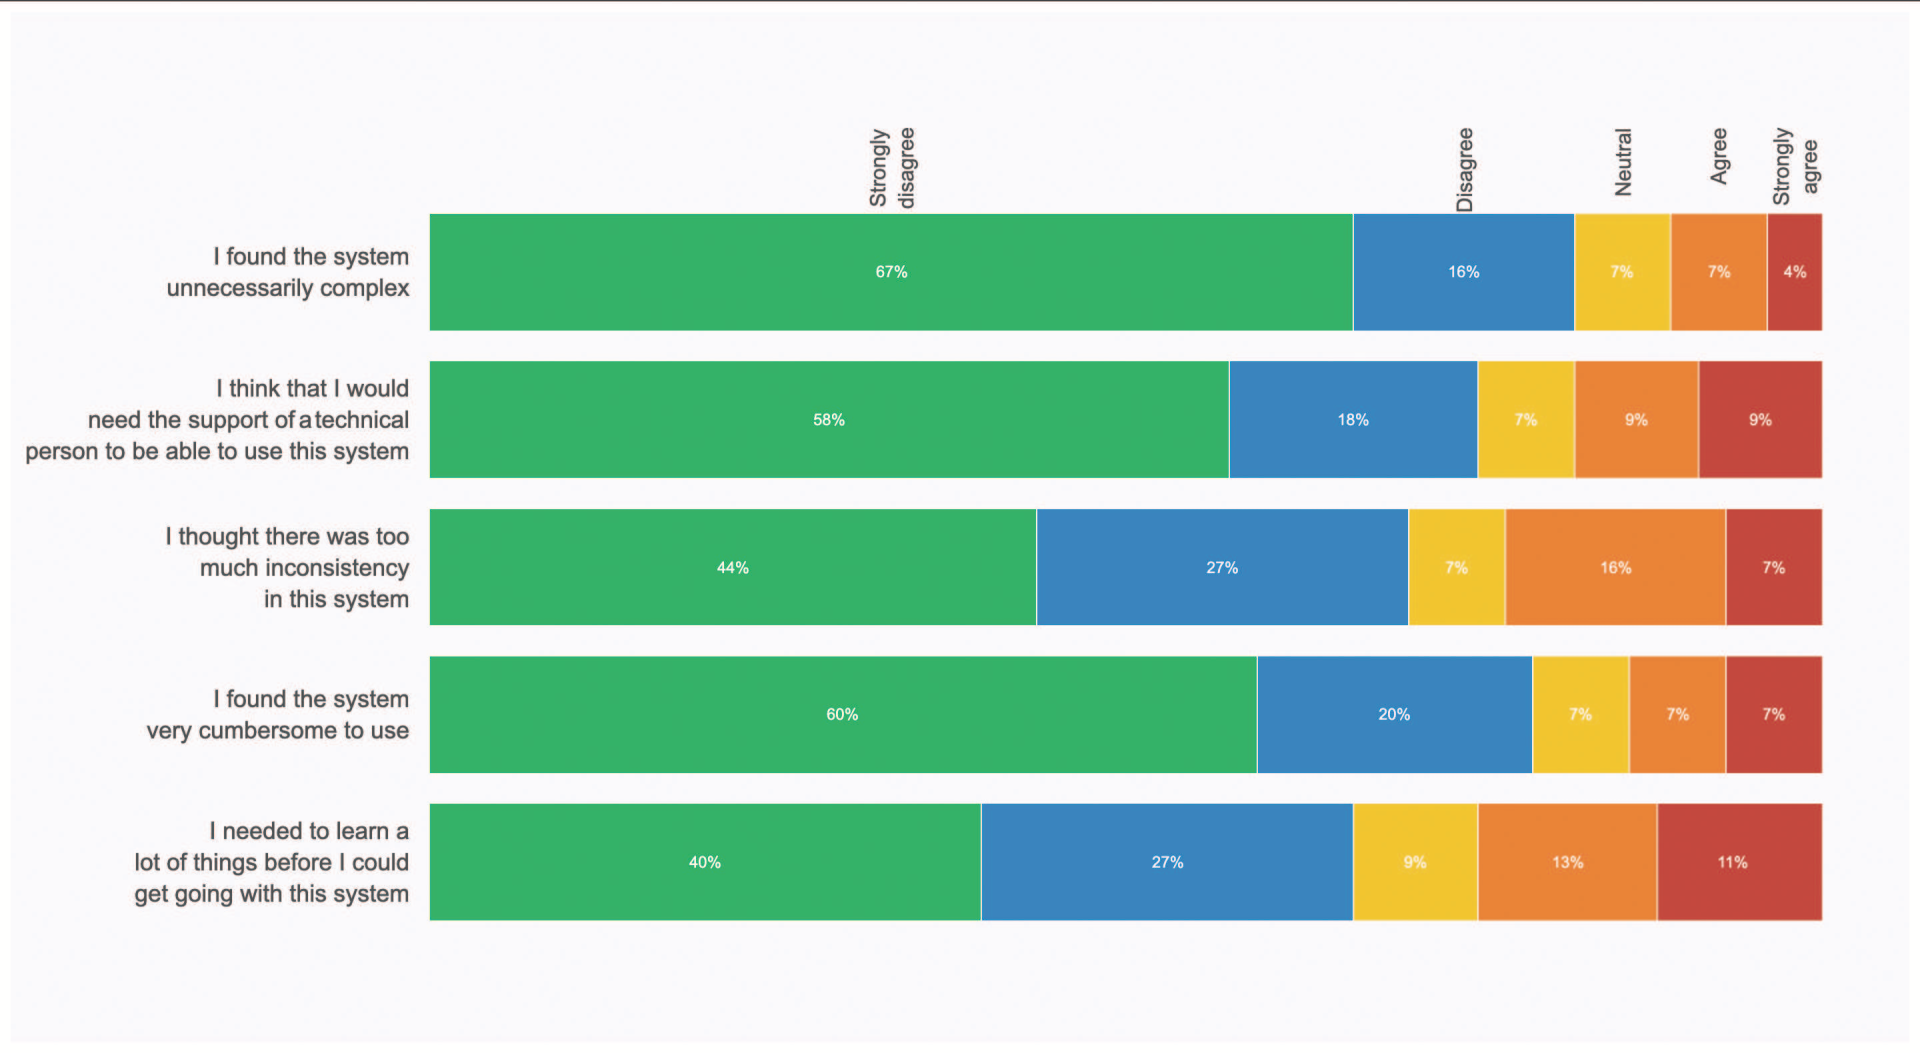
\includegraphics[width=\textwidth]{images/fig035}
\caption{Results of SUS with Negative Questions for the {\it Current} condition. In this case, it can be observed that 23\% found the system inconsistent and 24\% felt that need to learn before interacting with the system.}
\label{fig:fig035}
\end{figure}
%%%%%%%%%%%%%%%%%%%%%%%%%%%%%%%%%%%%%%%%%%%%%%%%%%%

%%%%%%%%%%%%%%%%%%%%%%%%%%%%%%%%%%%%%%%%%%%%%%%%%%%
\begin{figure}[htbp]
\centering
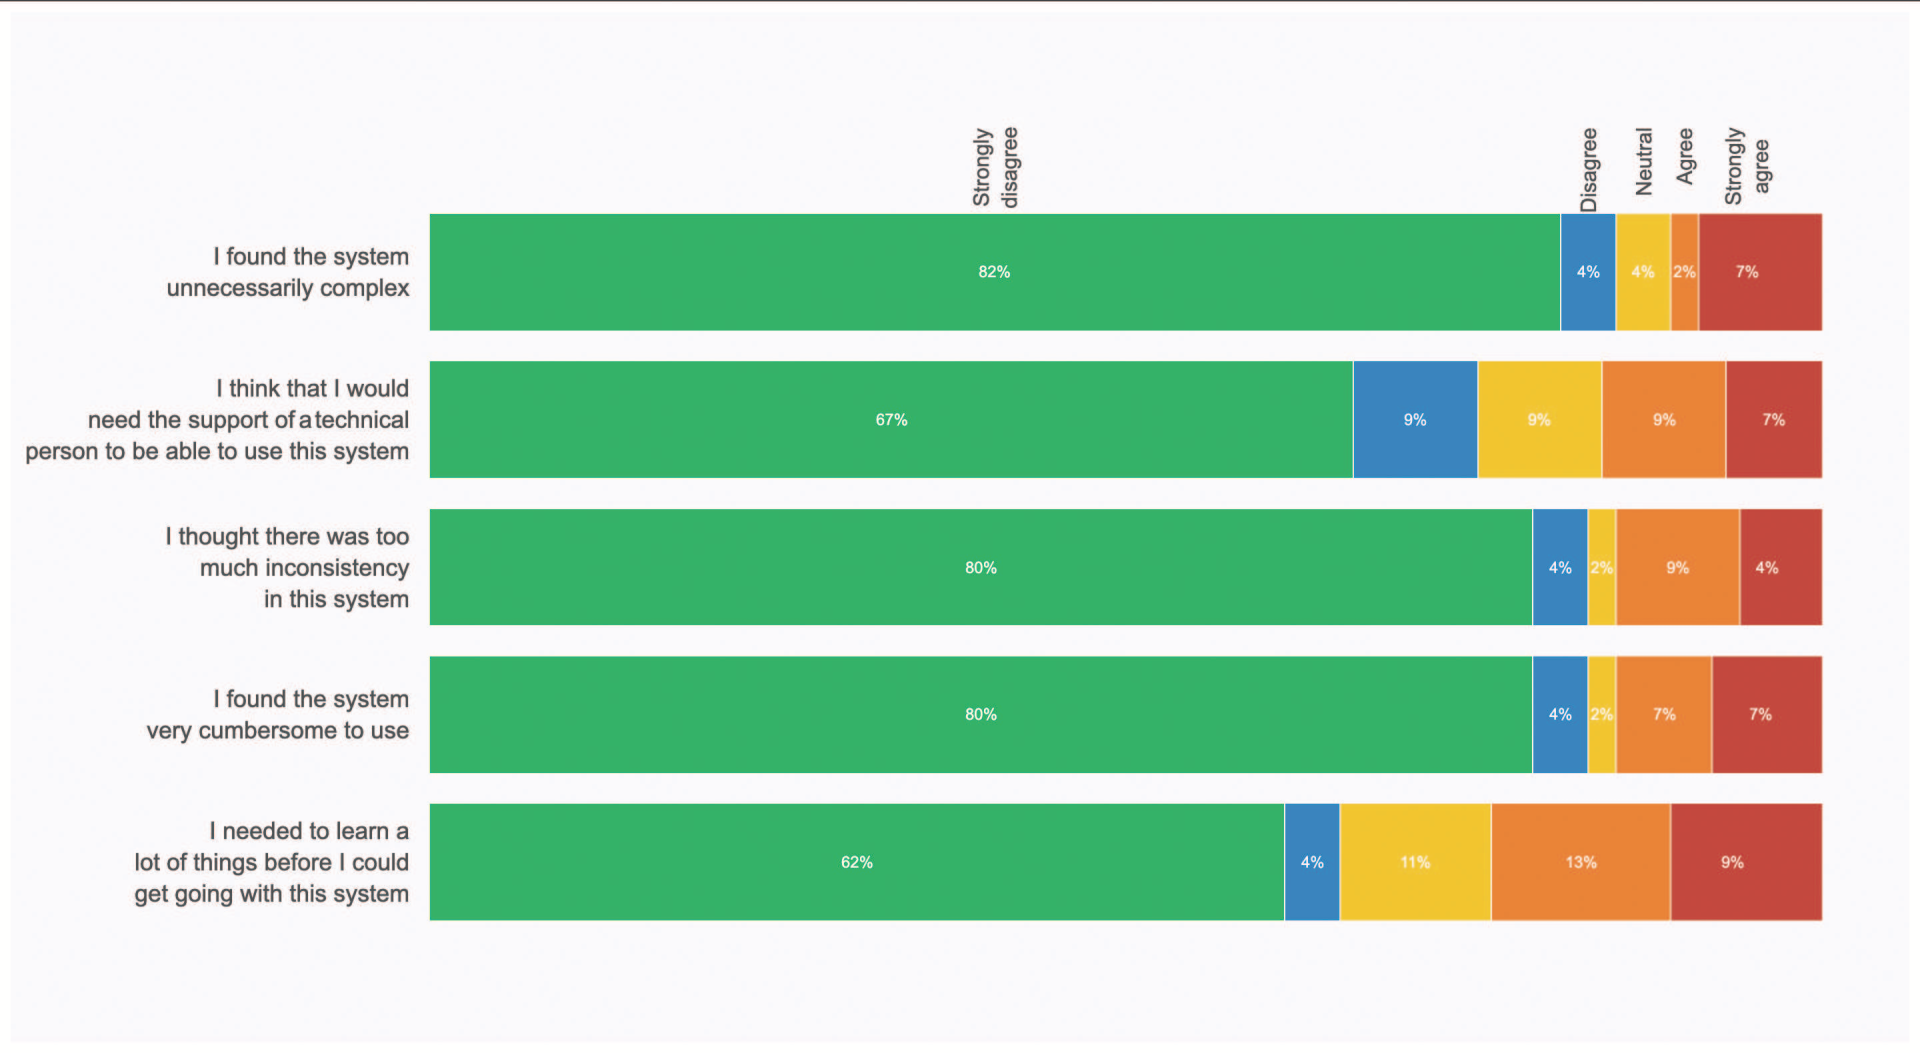
\includegraphics[width=\textwidth]{images/fig036}
\caption{Results of SUS with Negative Questions for the {\it Assistant} condition. Comparing the {\it Assistant} with the {\it Current} condition, it can be observed that clinicians found the {\it Assistant} condition less complex, inconsistent and cumbersome.}
\label{fig:fig036}
\end{figure}
%%%%%%%%%%%%%%%%%%%%%%%%%%%%%%%%%%%%%%%%%%%%%%%%%%%

\subsubsection{{\it Workload} (Demands)}
\label{sec:sec005006001003}

The results generated from the \ac{NASA-TLX}~\cite{ramkumar2017using, grier2015high} (Mental, Physical and Temporal) Demands are expressed in Table \ref{tab:tab001}.
For each \ac{NASA-TLX} item, the normalized data were first ranked and aligned to the \ac{ANOVA}\footnotemark[27] measurements.
There are two main conditions, {\it i.e.}, the {\it Current} (Curre.) condition and {\it Assistant} (Assis.) condition.
As follows, results are presented for the demands of the \ac{NASA-TLX} questionnaires.

%%%%%%%%%%%%%%%%%%%%%%%%%%%%%%%%%%%%%%%%%%%%%%%%%%%
\footnotetext[27]{{\it N}: the number of users (Clinicians); $F\textsubscript{var}$: the F-test used for comparing the factors of the total deviation per each variable ({\it var}) categorized by clinical experience; $M\textsubscript{var}$: Mean value of the variable ({\it var}); $SD\textsubscript{var}$: the Standard Deviation (SD) per each variable ({\it var}). Notice that from the statistical significance analysis described in Table \ref{tab:tab001} and setting a significance threshold to 0.05, two scenarios are possible to occur. First, if a p-value $>$ 0.05 is obtained, this means that the approaches are not statistically different, better saying. Thus, it can not state anything about the data. On the contrary, if the p-value $<$ 0.05 the approaches are statistically different, since now the value can reject the null hypothesis that states there is not a statistically significant difference between results of the proposed method and the other methods compared.}
%%%%%%%%%%%%%%%%%%%%%%%%%%%%%%%%%%%%%%%%%%%%%%%%%%%

%%%%%%%%%%%%%%%%%%%%%%%%%%%%%%%%%%%%%%%%%%%%%%%%%%%
\begin{table}[htbp]
\begin{tabular*}{\textwidth}{ c @{\extracolsep{\fill}} c c @{\extracolsep{\fill}} c c @{\extracolsep{\fill}} c c }
\toprule
\\
\small
&
\multicolumn{2}{ c }{Mental Demand}
&
\multicolumn{2}{ c }{Physical Demand}
&
\multicolumn{2}{ c }{Temporal Demand}
\\
\cmidrule(lr){2-3}
\cmidrule(lr){4-5}
\cmidrule(lr){6-7}
Condition & F & Sig. & F & Sig. & F & Sig. \\
\\
\bottomrule
\\
Current & 3.392 & 0.027$\star$ & 11.99 & 0.001$\star$ & 10.51 & 0.001$\star$ \\
Assistant & 0.638 & 0.594 & 2.852 & 0.048$\star$ & 0.035 & 0.991 \\
\\
\bottomrule
\hfill
\end{tabular*}
\caption{The ANOVA factorial analysis table regarding NASA-TLX for {\it Mental Demand (MD)}, {\it Physical Demand (PD)} and {\it Temporal Demand (TD)}, where {\it F} is the variation between sample means and the variation within samples. To determine whether any of the differences between the means are statistically significant, the {\it Sig.} was used for significance. On the present study, a 20-point Likert Scale was used regarding Workload. The factorial analysis was described assuming $\alpha = 0.05$. Also, each time $p < 0.05$ it is marked with the $\star$ symbol.}
\label{tab:tab001}
\end{table}
%%%%%%%%%%%%%%%%%%%%%%%%%%%%%%%%%%%%%%%%%%%%%%%%%%%

The \ac{ANOVA} statistical test~\cite{Wobbrock:2011:ART:1978942.1978963, mathews2017usability} yields a significant main effect for the Mental Demand (F\textsubscript{Curre.} = 3.39, p\textsubscript{Curre.} = 0.027 $<$ 0.05), Physical Demand (F\textsubscript{Curre.} = 11.99, p\textsubscript{Curre.} = 0.001 $<$ 0.05) and Temporal Demand (F\textsubscript{Curre.} = 10.51, p\textsubscript{Curre.} = 0.001 $<$ 0.05).
On the other hand, the {\it Assistant} condition indicates a significant difference only in Physical Demand (F\textsubscript{Assis.} = 2.85, p\textsubscript{Assis.} = 0.048 $<$ 0.05). A detailed comparison is shown in Table~\ref{tab:tab001}.
Despite of the higher rates from the \ac{NASA-TLX} over the several Demands (Table~\ref{tab:tab001}), it can be pointed improvements from the {\it Current} to the {\it Assistant} setup.

From this study, it can be identified that some functionalities contribute significantly to one (or more) types of workloads (criteria variables) in the \ac{NASA-TLX} questionnaire.
For instance, increasing the number of available image modalities on the viewport is strongly associated to Mental Demand.
However, for the {\it Assistant} condition it is not possible to take conclusions since the fact that their is no significant main effect.
The overall time duration of manipulating the images ({\it i.e.}, zoom, pan, scroll) is strongly associated to the Physical Demand.
Comparing both {\it Current} and {\it Assistant} conditions, it is possible to be observed a significant main effect and improvements on the {\it Assistant} condition.

The time duration of decision-making is strongly associated with Temporal Demand.
Nonetheless, only the {\it Current} condition follows a significant main effect making it difficult to do a strong comparison with the {\it Assistant} condition.
For simplicity of the results, this work divided the \ac{NASA-TLX} questionnaire items in {\bf Demands} and {\bf Non-Demands} categories.
Next (Section~\ref{sec:sec005006001004}), the document will report the three items from {\bf Non-Demands} of the \ac{NASA-TLX} questionnaire.

\subsubsection{{\it Workload} (Non-Demands)}
\label{sec:sec005006001004}

The \ac{NASA-TLX} on the Non-Demands scales only yields significant difference among groups for Performance (F\textsubscript{Curre.} = 5.56, p\textsubscript{Curre.} = 0.003 $<$ 0.05).
A more detailed comparison is shown on Table~\ref{tab:tab002}.
Despite these higher rates, one can point improvements from {\it Current} vs {\it Assistant}.

%%%%%%%%%%%%%%%%%%%%%%%%%%%%%%%%%%%%%%%%%%%%%%%%%%%
\begin{table}[htbp]
\begin{tabular*}{\textwidth}{ c @{\extracolsep{\fill}} c c @{\extracolsep{\fill}} c c @{\extracolsep{\fill}} c c }
\toprule
\\
\small
&
\multicolumn{2}{ c }{Effort}
&
\multicolumn{2}{ c }{Performance}
&
\multicolumn{2}{ c }{Frustration}
\\
\cmidrule(lr){2-3}
\cmidrule(lr){4-5}
\cmidrule(lr){6-7}
Condition & F & Sig. & F & Sig. & F & Sig. \\
\\
\bottomrule
\\
Current & 0.534 & 0.661 & 5.556 & 0.003$\star$ & 2.392 & 0.082 \\
Assistant & 0.664 & 0.578 & 0.319 & 0.811 & 0.408 & 0.748 \\
\\
\bottomrule
\hfill
\end{tabular*}
\caption{ The ANOVA factorial analysis table regarding NASA-TLX for \textit{Effort (Eff.)}, \textit{Performance (Per.)} and \textit{Frustration (Fru.)}, where {\it F} is the variation between sample means and the variation within samples. To determine whether any of the differences between the means are statistically significant, the {\it Sig.} for significance was used. On the present study, a 20-point Likert Scale was used regarding Workload. The factorial analysis was described assuming $\alpha = 0.05$. Also, each time $p < 0.05$ it is marked with the $\star$ symbol.}
\label{tab:tab002}
\end{table}
%%%%%%%%%%%%%%%%%%%%%%%%%%%%%%%%%%%%%%%%%%%%%%%%%%%

This is a result of the increasing number of visualization modalities, from one in the {\it Current} condition, to three in the {\it Assistant} condition while it is assisted by an \ac{AI} model.
Due to the fact that in {\it Current} condition clinicians are analyzing less number of lesions, the effort is less in comparison to the {\it Assistant} condition.
For the {\it Current} condition results, clinicians just diagnosed one modality per each ({\it i.e.}, {\bf P1}, {\bf P2} and {\bf P3}) patient.
On the contrary, for the {\it Assistant} results, each clinician diagnose all the three modalities ({\it i.e.}, \ac{MG}, \ac{US} and \ac{MRI}) per each patient.
In fact, the improvement scores (\textbf{F}) of the proposed {\it Assistant} are positive.
Note that, as far as the scores are less than three times the results from the {\it Current} condition, one can conclude that it is getting better results.

Effort and Frustration do not provide any significant main effect on both {\it Current} and {\it Assistant} conditions.
Therefore, it is not possible to consider any findings regarding these issues.
Nor even the Performance results, since the fact that the {\it Assistant} does not represent any significant main effect.
Notwithstanding, these results will be paired (Section~\ref{sec:sec005006}) with the above (Demands) and these (Non-Demands) \ac{NASA-TLX} results with other metrics to discuss the final results with more evidence.

\subsubsection{{\it Diagnostic Time} vs {\it Breast Severity}}
\label{sec:sec005006001005}

The results\footnotemark[28] expressing the full diagnostic time length and breast severity among the 289 Patients ({\it i.e.}, {\bf P1} - Low, {\bf P2} - Medium and {\bf P3} - High severities) are shown in Figure \ref{fig:fig037}.
For the {\bf P1} - Low severity, the {\it Current} (M\textsubscript{Curre.} = 146, SD\textsubscript{Curre.} = 86.17) condition was longer than the {\it Assistant} (M\textsubscript{Assis.} = 89, SD\textsubscript{Assis.} = 74.13) condition.
However, for the {\bf P2} - Medium severity, the {\it Current} (M\textsubscript{Curre.} = 78, SD\textsubscript{Curre.} = 48.05) condition was, again, longer than the {\it Assistant} (M\textsubscript{Assis.} = 77, SD\textsubscript{Assis.} = 96.80) condition.
Finally, for the {\bf P3} - High severity, the {\it Current} (M\textsubscript{Curre.} = 116, SD\textsubscript{Curre.} = 65.70) condition was longer than the {\it Assistant} (M\textsubscript{Assis.} = 64, SD\textsubscript{Assis.} = 86.94) condition.
The \ac{ANOVA} statistical test shows a significant effect over the total {\it Time} for the {\it Current} (F\textsubscript{Curre.} = 3.25, p\textsubscript{Curre.} = 0.03 $<$ 0.05) condition regarding the clinical experience groups on a {\bf P1} - Low severity case.
Verifying that the introduction of an intelligent agent did not increase the diagnostic time for Low and High severities.

%%%%%%%%%%%%%%%%%%%%%%%%%%%%%%%%%%%%%%%%%%%%%%%%%%%
\footnotetext[28]{An available dataset (\href{https://mimbcd-ui.github.io/dataset-uta7-time/}{mimbcd-ui.github.io/dataset-uta7-time}) is provided and made public from the achieved {\it time} data. This will make the work more easier to replicate the results from the scientific community, or more precisely, for the HCI community. The link was accessed on 6th of December, 2020.}
%%%%%%%%%%%%%%%%%%%%%%%%%%%%%%%%%%%%%%%%%%%%%%%%%%%

%%%%%%%%%%%%%%%%%%%%%%%%%%%%%%%%%%%%%%%%%%%%%%%%%%%
\begin{figure}[ht]
\centering
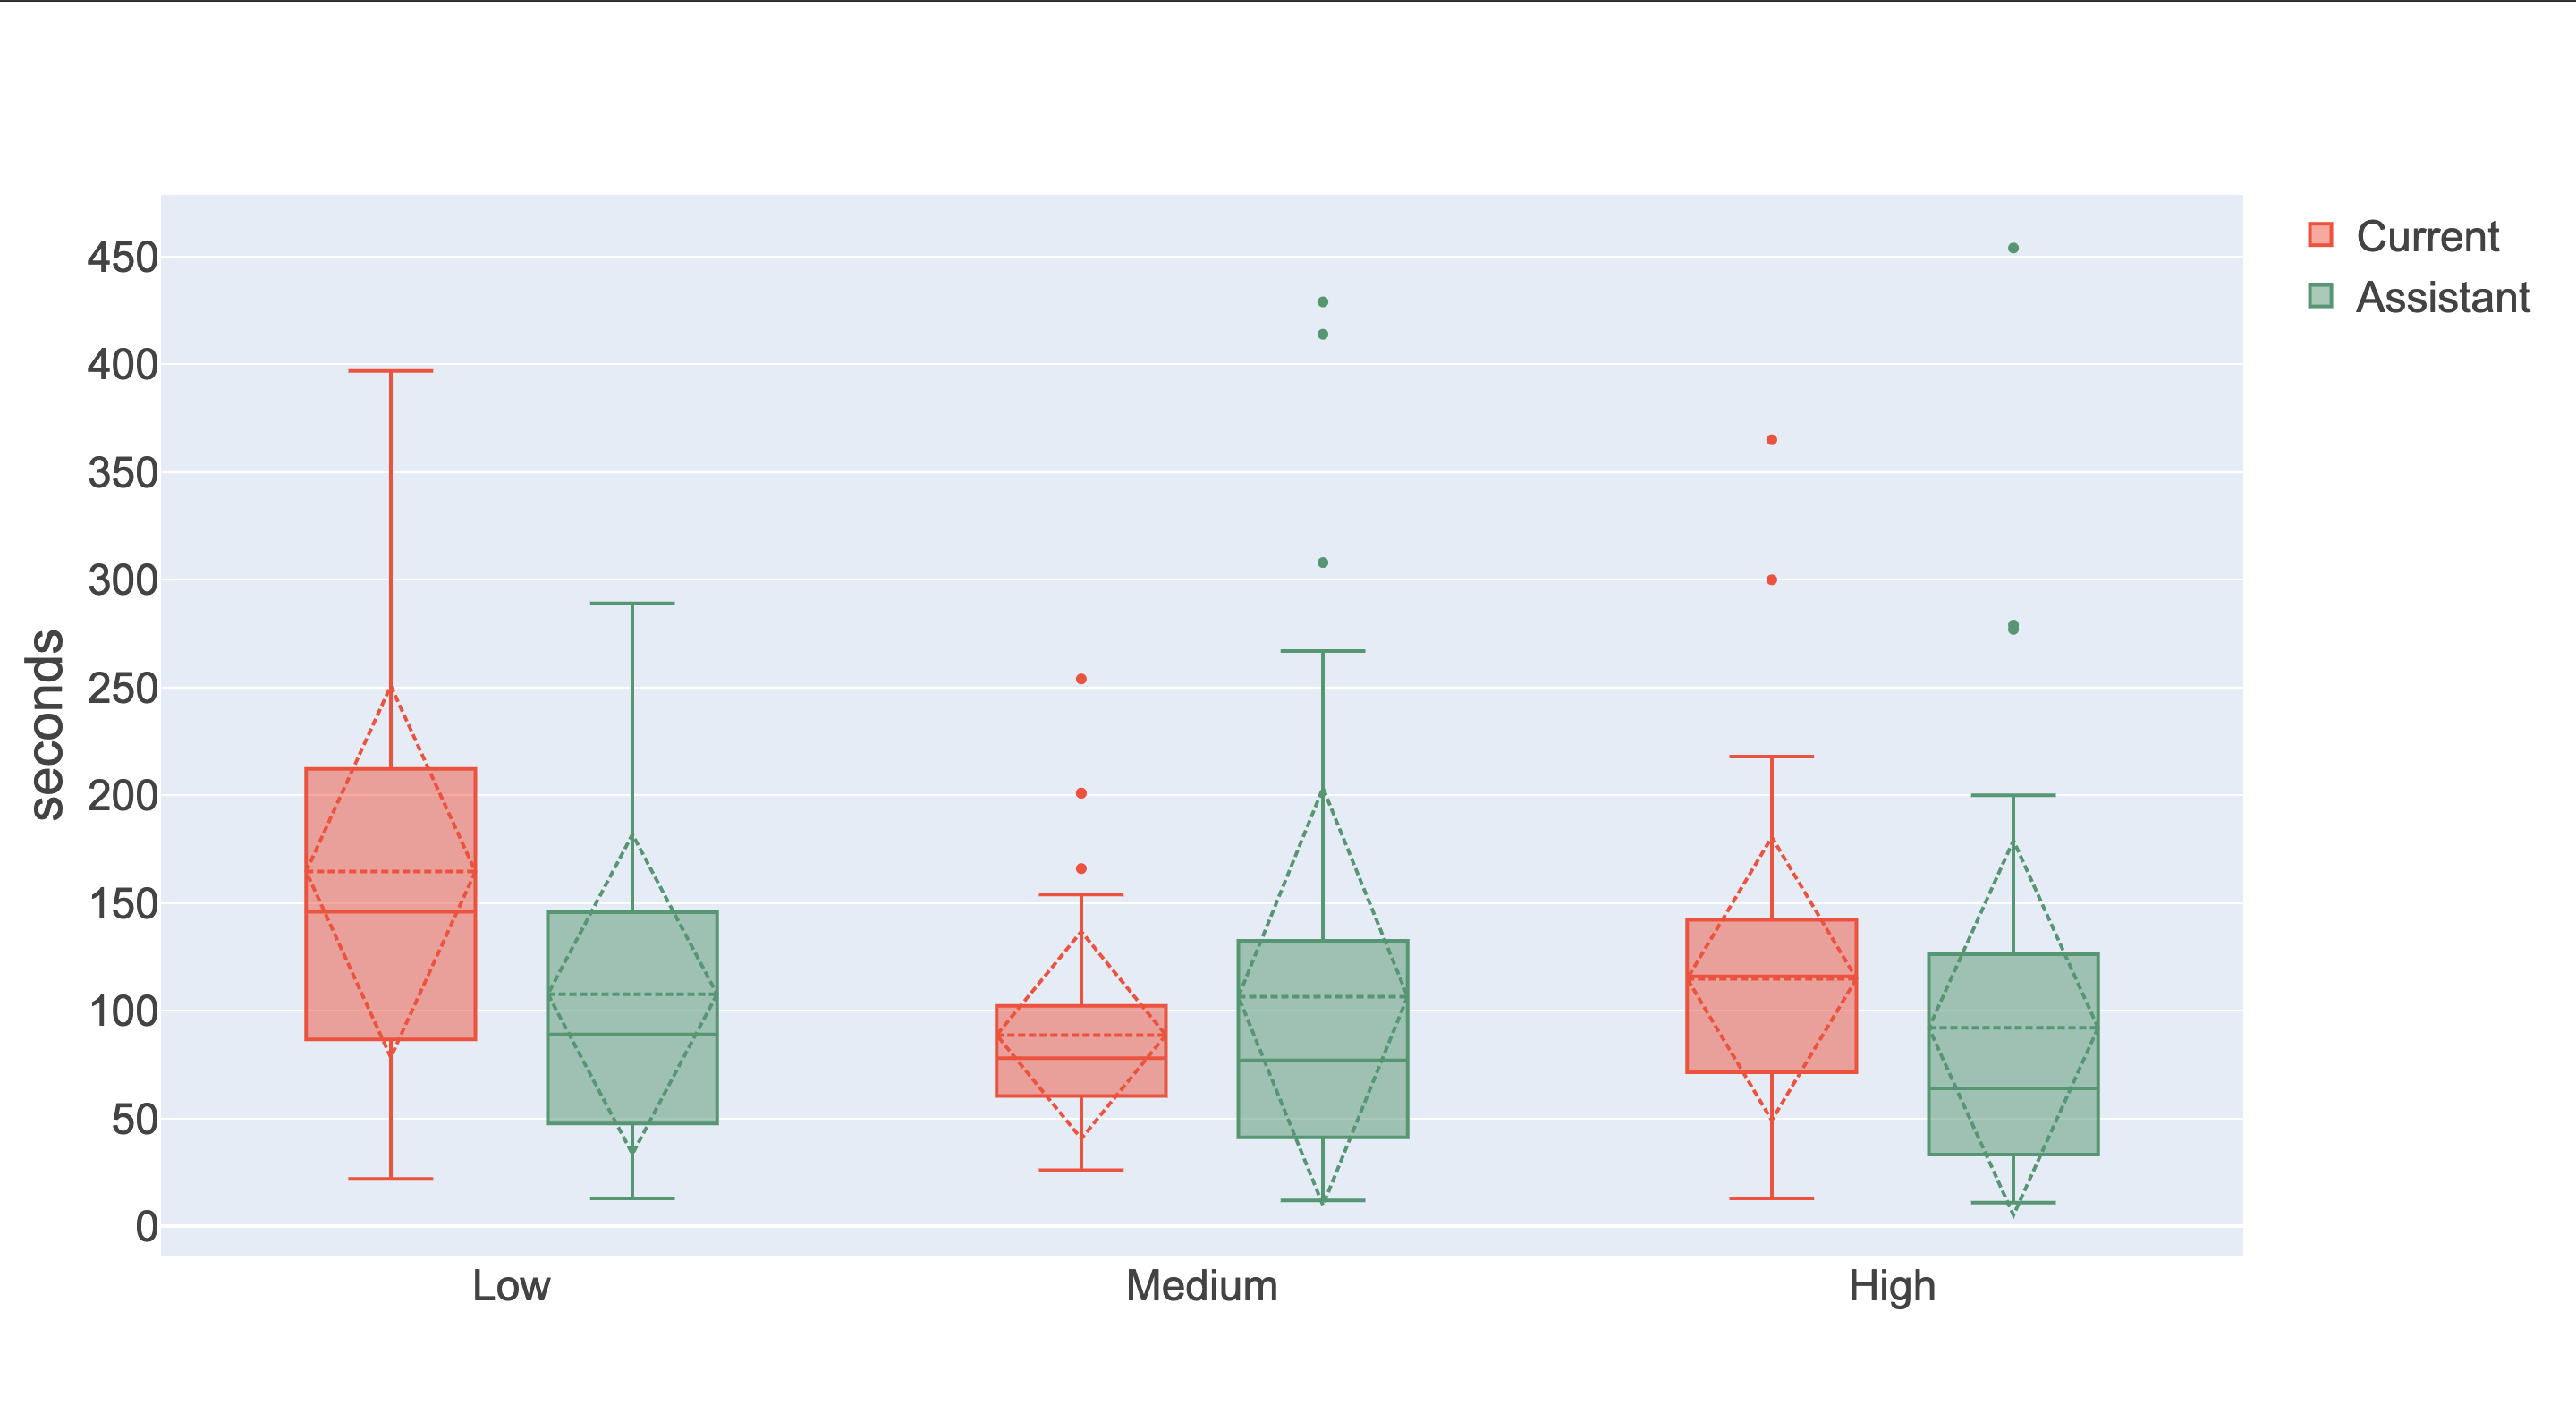
\includegraphics[width=\columnwidth]{images/fig037}
\caption{Relation between full diagnostic time length (seconds) and breast severity. Both {\it Current} (Curre.) condition and {\it Assistant} (Assis.) condition were compared as Low, Medium and High values of BI-RADS.}
\label{fig:fig037}
\end{figure}
%%%%%%%%%%%%%%%%%%%%%%%%%%%%%%%%%%%%%%%%%%%%%%%%%%%

Planned post-hoc testing~\cite{10.1145/2858036.2858360}, using the Tukey's HSD Post-Hoc Comparison (p\textsubscript{Curre.} $<$ 0.05), revealed that for the groups of {\it Juniors} it significantly increased the time performance and severity accuracy compared to {\it Interns}.
Therefore, the proposed intelligent agent, not only improves time performance (Figure~\ref{fig:fig037}) and diagnostic accuracy (Figure~\ref{fig:fig038}) among the others clinicians' categories of medical experience, but also provides important support for {\it Interns}.

Although the diagnostic time increased on medium severities, the increase was just residual and will be further discussed (Section~\ref{sec:sec005007}).
These results support {\bf RQ5.1}, suggesting that the proposed {\it BreastScreening-AI} tool could impact positively the clinical workflow.
While improving time performance (Section~\ref{sec:sec005006001005}) and diagnostic accuracy (Section~\ref{sec:sec005006001006}), the system is also mitigating the different types of errors on clinical perception.

\subsubsection{{\it False-Negatives} vs {\it False-Positives}}
\label{sec:sec005006001006}

In this study, it was also measured the rates of \acp{FN} and \acp{FP} (Figure~\ref{fig:fig038}) between {\it Current} and {\it Assistant} conditions.
The \ac{FN} rates decrease from 33\% on the {\it Current} condition to 14\% on the {\it Assistant} condition.
From the published dataset\footnotemark[29], the results show a significant potential reduction of \acp{FN}, i.e., cases where the diagnosis leads to a low severity (\ac{BI-RADS}) against expert ground-truth.

%%%%%%%%%%%%%%%%%%%%%%%%%%%%%%%%%%%%%%%%%%%%%%%%%%%
\footnotetext[29]{Under this work, an available dataset (\href{https://mimbcd-ui.github.io/dataset-uta7-rates/}{mimbcd-ui.github.io/dataset-uta7-rates}) concerning the severity {\it rates} (BI-RADS) was provided. The link was accessed on 6th of December, 2020.}
%%%%%%%%%%%%%%%%%%%%%%%%%%%%%%%%%%%%%%%%%%%%%%%%%%%

%%%%%%%%%%%%%%%%%%%%%%%%%%%%%%%%%%%%%%%%%%%%%%%%%%%
\begin{figure}[ht]
\centering
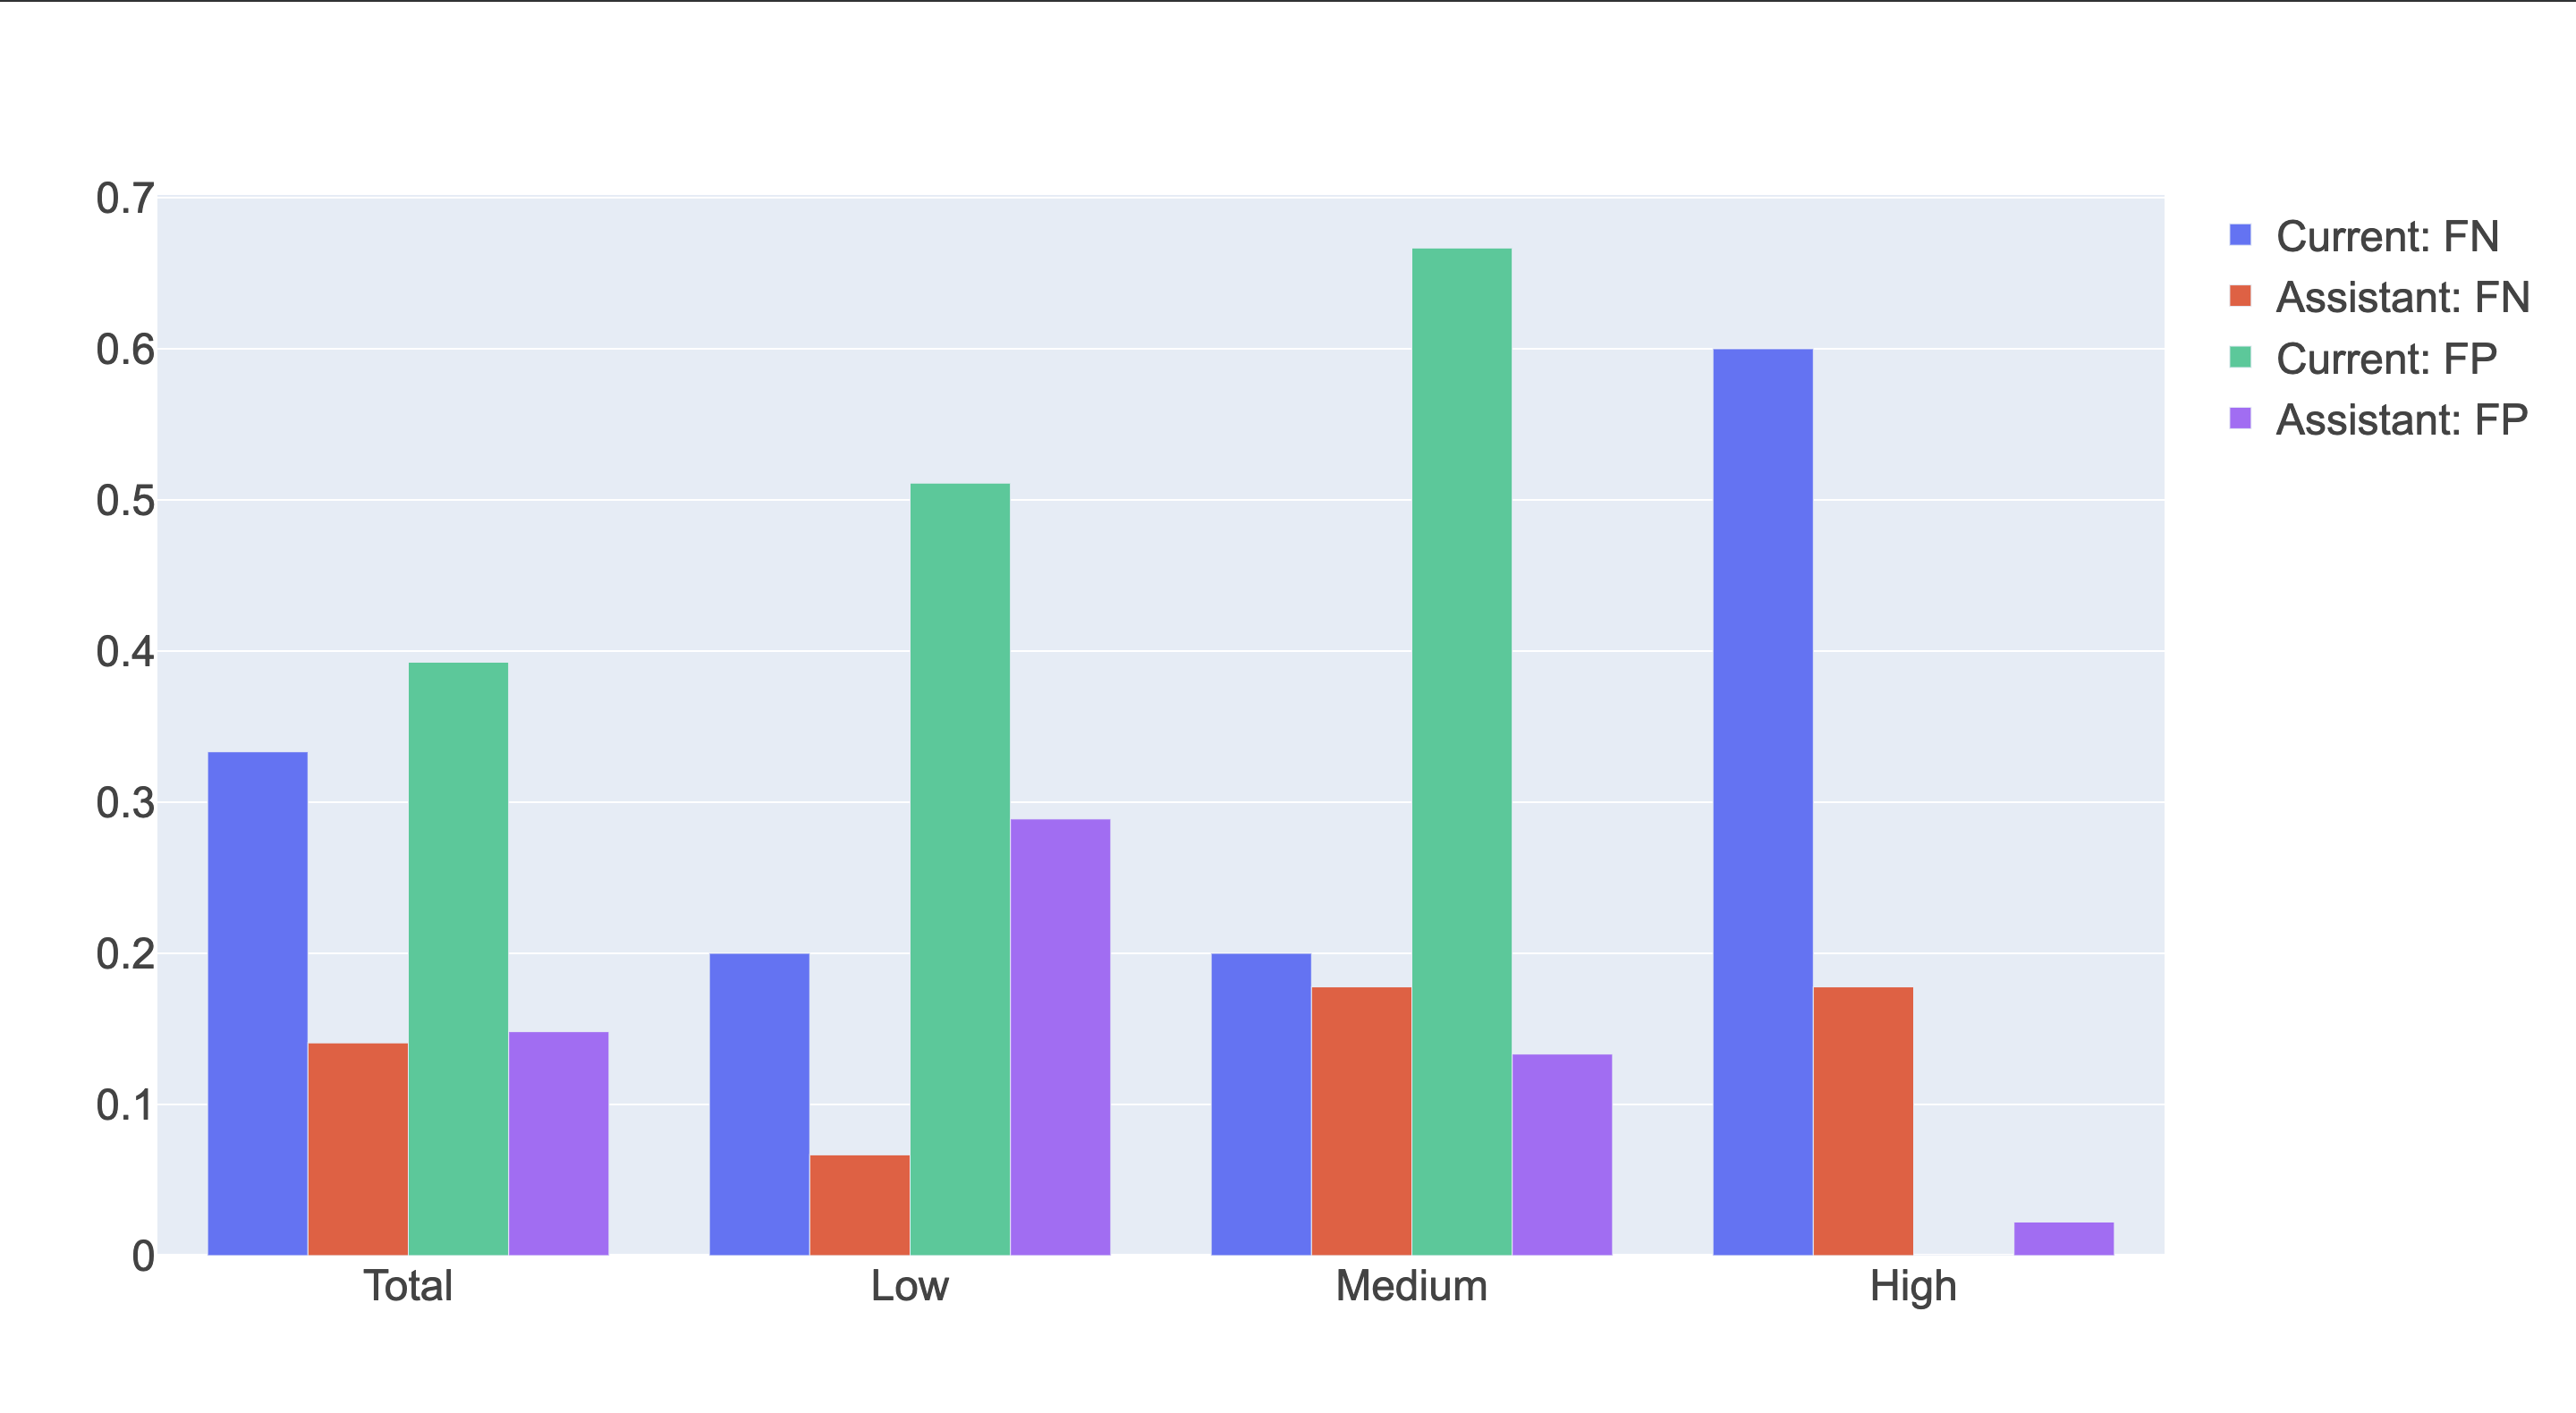
\includegraphics[width=\columnwidth]{images/fig038}
\caption{{\it Current} {\bf vs} {\it Assistant} rates for False-Negatives and False-Positives. A False-Positive is considered when the BIRADS\textsubscript{provided} $>$ BIRADS\textsubscript{real}. A False-Negative is considered when the BIRADS\textsubscript{provided} $<$ BIRADS\textsubscript{real}.}
\label{fig:fig038}
\end{figure}
%%%%%%%%%%%%%%%%%%%%%%%%%%%%%%%%%%%%%%%%%%%%%%%%%%%

Notwithstanding, the \ac{FP} rates decrease from 39\% on the {\it Current} condition to the 15\% on the {\it Assistant} condition for an overall ({\it i.e.}, Total) condition.
In essence, the intelligent agent will have a 24\% decrease of situations where clinicians are providing a \ac{BI-RADS} higher than the real one.
These results are paired with the results of Chapter~\ref{chap:chap006}, where a more detailed study is making further claims of the achieved \acp{FP} and \acp{FN} rates in a more descriptive manner.

\subsection{Qualitative Analysis}
\label{sec:sec005006002}

In this study, quantitative analysis are completed with insights and results from interviewing participants.
In this section, the study of a preliminary design is described for the development of the prosed {\it Assistant}, informed by an iterative process to identify clinician's needs and recommendations.
First of all, from a set of workshops (Section~\ref{sec:sec005006002001}) participants were introduced to aspects or open-ended questions that can drive this initial stage of qualitative data analysis.
In this workshops, participants are divided into small groups.
Second, by joining the research team with participants, the focus group (Section~\ref{sec:sec005006002002}) sessions are established.
And third, to cluster and categorize (Section~\ref{sec:sec005006002003}) the set ideas, features and priorities, in this focus group it was introduced a lightweight approach called affinity diagrams (Section~\ref{sec:sec005006002004}).
The following sections will detail and describe this qualitative analysis.

\subsubsection{Workshops with Clinicians}
\label{sec:sec005006002001}

The first step of our methodology was to record {\it workflow} practices and routines from clinicians~\cite{Hoiseth:2013:DHG:2485760.2485770, Hoiseth:2013:RGD:2468356.2468436}.
To this end, several invitations were sent among the various medical institutions and, at least, one workshop was formed per each institution as described next.
All participants, that volunteer to the remain study, were grouped in various sessions.
The research team went to these clinical institutions (Section~\ref{sec:sec005005001}) at least one day per each institution.
For Hospital Fernando Fonseca, four workshop meetings were made, while it was the institution with more clinicians and, therefore, harder to schedule.
For IPO Lisboa, two workshop meetings were made, as well as for Hospital do Barreiro.
For the other institutions, just one workshop meeting was made.
A total of 45 professionals from the sector of healthcare ({\it i.e.,} Radiologists, Oncologists and Surgeons), as well as six members of the {\it BreastScreening} research work ({\it i.e.}, \ac{HCI} and \ac{AI} Researchers) participated in these series of workshops.

Based on preliminary content analysis of the semi-structured interviews with clinicians, workshops were conducted as part of the {\it BreastScreening} research work development.
Participants worked in groups and brainstormed around their clinical practices and routines.
Most of the practices are recorded and written.
Also, notes were digitally transcribed while addressing (Section~\ref{sec:sec005006002003}) the affinity diagramming\footnotemark[30] technique.

%%%%%%%%%%%%%%%%%%%%%%%%%%%%%%%%%%%%%%%%%%%%%%%%%%%
\footnotetext[30]{Affinity diagramming is a powerful method for performing qualitative data organization and analysis. The method was used to help understand the role of technology into the radiology room workflow. More precisely, affinity diagrams were used to organize the provided information from clinicians to group it with related ideas or topics.}
%%%%%%%%%%%%%%%%%%%%%%%%%%%%%%%%%%%%%%%%%%%%%%%%%%%

The duration of workshop by session was roughly two hours, and ended with joint sessions wherein each group of clinicians highlighted important aspects of the clinical {\it workflow} for their institutions.
At the end of the workshop sessions, four different procedures were collected (Figure \ref{fig:fig018}) of acquiring medical images.
Participants engaged into the planed design activities~\cite{https://doi.org/10.13140/rg.2.2.16566.14403/1}, in which they provided inputs regarding the current {\it Assistant}.
Using the provided input from the workshops, a prototype was designed which was evaluated during several sessions at the nine (Section~\ref{sec:sec005005001}) clinical institutions.

\subsubsection{Focus Groups}
\label{sec:sec005006002002}

Building on the qualitative data from the workshops with clinicians, a focus group consisting of six Researchers (MSc, PhD and Post-Doc students, as well as Assistant and Full Professors) and another six Radiologists (2 seniors; 1 middle; 2 juniors; and 1 intern) from Hospital Fernando Fonseca, organized the {\it workflow} practices and main feature ideas to greater detail by using affinity diagrams~\cite{Harboe:2012:CSC:2145204.2145379, Hoiseth:2013:RGD:2468356.2468436}.

The affinity diagrams enable this study to identify several functionalities, such as the need to {\it accept} or {\it reject} (Figure~\ref{fig:fig031}) the {\it Assistant} result.
Also important, it was from the affinity diagrams that it was achieved a high priority feature for developing a technique so that in case of {\it reject} the {\it Assistant} result, the clinician can provide new information to the DenseNet.

\hfill

\noindent
This technique is novel and, while applying these \ac{HCI} practices, it provides a twofold of contributions:

%%%%%%%%%%%%%%%%%%%%%%%%%%%%%%%%%%%%%%%%%%%%%%%%%%%
\begin{enumerate}
\item Creating a new way of control on the introduction of \ac{AI} methods, via intelligent agents. among medical imaging diagnosis; and
\item The inclusion of a \ac{DNN} in the \ac{UI} with a form of an intelligent agent, particularly, the introduction of a pre-trained DenseNet capable to provide a fast and reliable classification. To the best of the current knowledge, this is the first attempt to include in the \ac{UI} a feedback coming from a \ac{DNN} in breast cancer diagnosis.
\end{enumerate}
%%%%%%%%%%%%%%%%%%%%%%%%%%%%%%%%%%%%%%%%%%%%%%%%%%%

Another important aspect coming from these focus groups is that the \ac{MG} image modality is always present on a first stage of medical image acquisition, mainly because of its low cost.
The \ac{US} is the second most preferred modality to cross information between \ac{MG} image modality views ({\it i.e.}, \ac{CC} or \ac{MLO}).
Finally, because of the high costs ({\it e.g}, time of acquiring the images) associated with the \ac{MRI}, clinicians said (in nine institutions only one follows the {\bf Proc. 4}, see Figure \ref{fig:fig018}) it was typically recommended only for highly risk patients.

\subsubsection{Affinity Diagrams}
\label{sec:sec005006002003}

This was an interactive process that consisted of adding or removing items until a final pattern configuration is reached.
As these ideas and functionalities from the clinicians could be relevant for several purposes, it was considered useful to short on a more general level to start with.
Ideas, features and priorities were translated (Figure~\ref{fig:fig039}) to a digital tool\footnotemark[31], while the affinity diagrams~\cite{10.1145/3290605.3300628} are used for: (i) categorization of the focus group items; and (ii) data clustering of the chaotic information.
This solves the problem (Section~\ref{sec:sec005006002004}) of chaotic data~\cite{10.1145/2858036.2858373, 10.1145/3343413.3377983} disorganization.

%%%%%%%%%%%%%%%%%%%%%%%%%%%%%%%%%%%%%%%%%%%%%%%%%%%
\footnotetext[31]{For that, the collaboration software Trello was used, which allowed this study to digitally organize and manage the group ideas. (\href{https://trello.com}{trello.com})}
%%%%%%%%%%%%%%%%%%%%%%%%%%%%%%%%%%%%%%%%%%%%%%%%%%%

%%%%%%%%%%%%%%%%%%%%%%%%%%%%%%%%%%%%%%%%%%%%%%%%%%%
\begin{figure}[htbp]
\centering
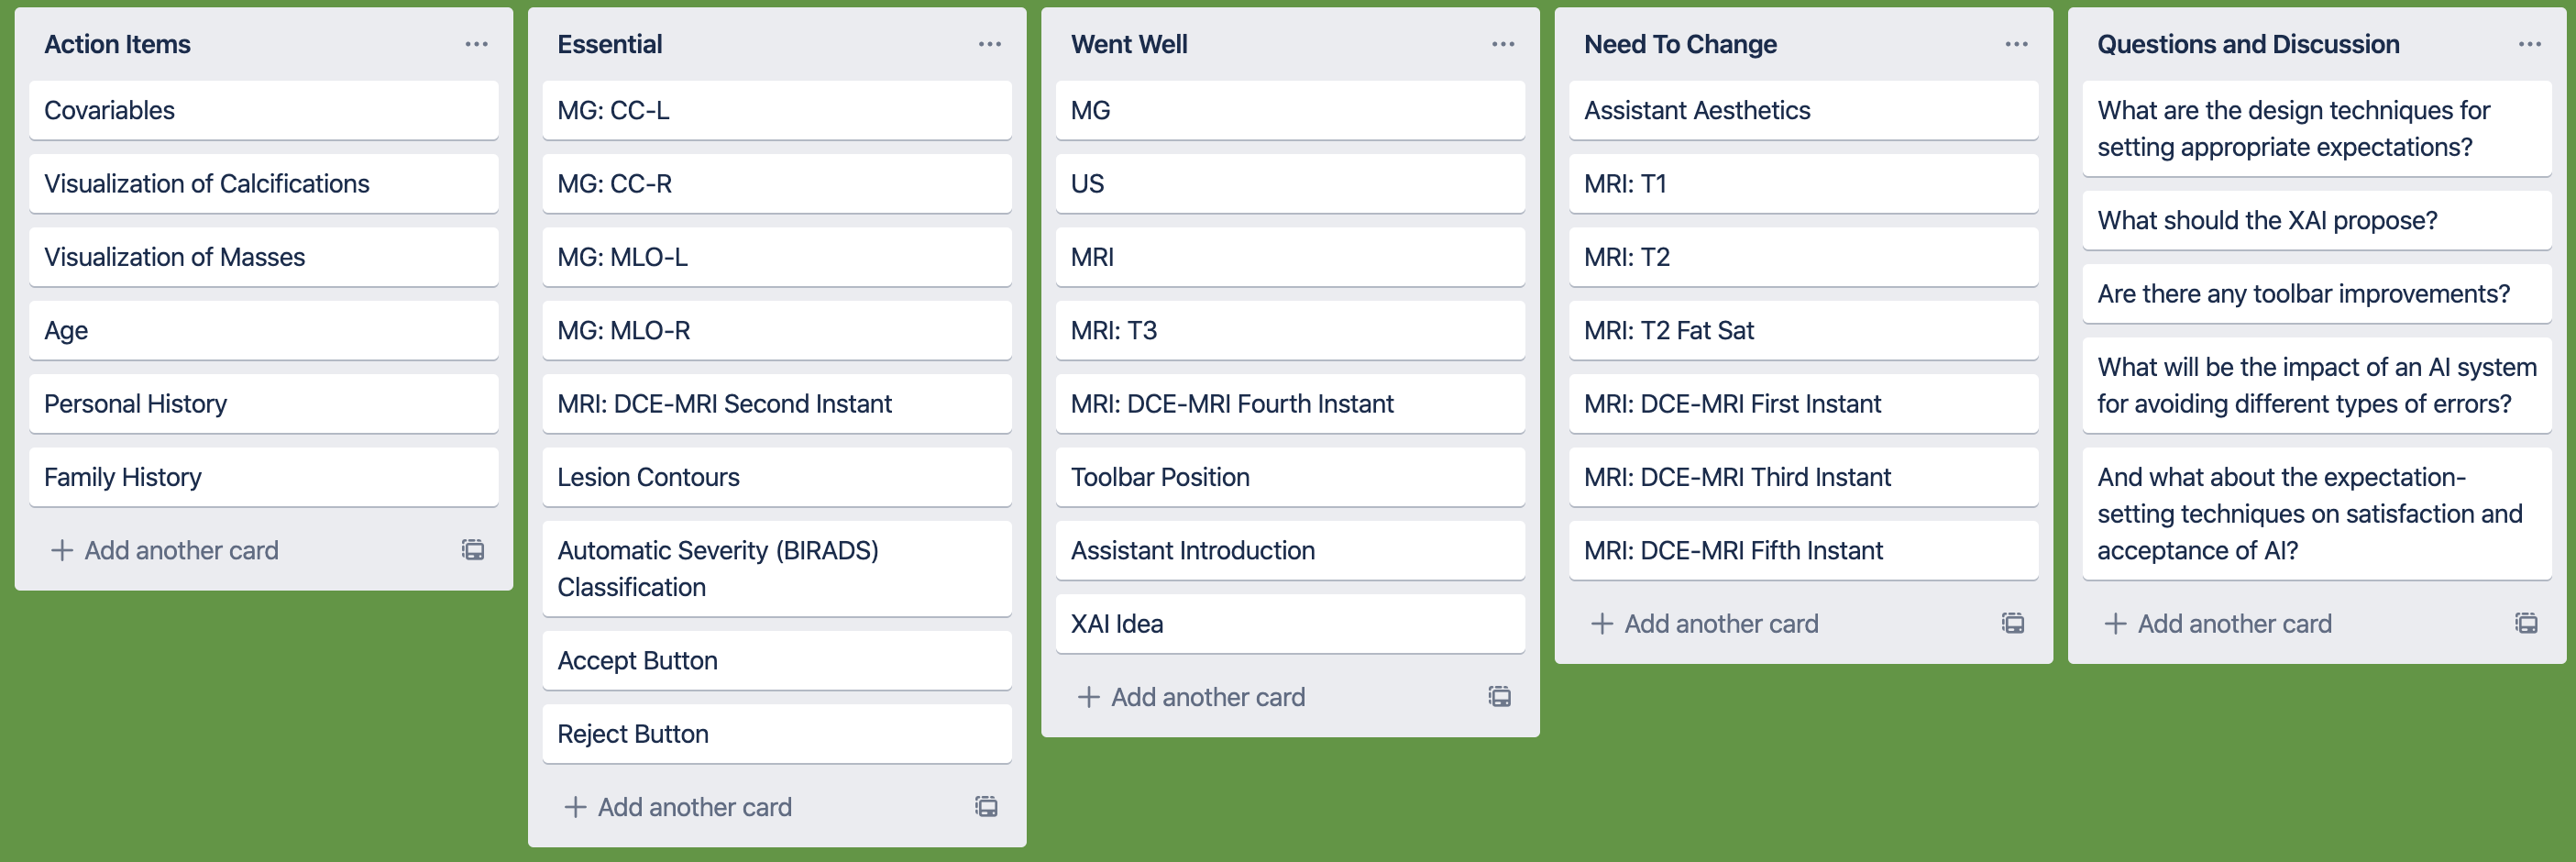
\includegraphics[width=\columnwidth]{images/fig039}
\caption{Resulting affinity diagrams passed to a digital software tool. The overall ideas and features categorization. Each idea and feature has a category ({\it e.g.}, "Action Items", "Essential", "Went Well", "Need To Change" or "Questions and Discussion"), so that it can manage the final requirements and development priorities of the {\it Assistant}.}
\label{fig:fig039}
\end{figure}
%%%%%%%%%%%%%%%%%%%%%%%%%%%%%%%%%%%%%%%%%%%%%%%%%%%

From workshops (Section~\ref{sec:sec005006002001}), participants ({\it i.e.}, researchers and some of the clinicians) of the focus group (Section~\ref{sec:sec005006002002}), were asked to review and re-position ideas and functionalities, within each category, in order to organize them.
Every time an idea or a functionality was triggered, it was inserted on the ``Action Items'' category.
After that, participants discuss where it should be, answering the workshop needs for item categorization.
For instance, several clinicians listed\footnotemark[32] their preferred components as the position (32/45) and simplicity (28/45) of the {\it Toolbar} (Section~\ref{sec:sec004003001003} and Section~\ref{sec:sec005004002}):
``The {\it Toolbar} position is in a better place on the top in contrary what we usually [Current] see'' (C30).
From here, an item was created titled as ``Toolbar Position'' and since it was accepted by a major number of clinicians (and rejected or omitted by another number) the item was stuck onto the ``Went Well'' category.

%%%%%%%%%%%%%%%%%%%%%%%%%%%%%%%%%%%%%%%%%%%%%%%%%%%
\footnotetext[32]{The workshop answers and feedback were transcribed so that they can join with similar opinions in different items. A ``(32/45)'' means that 32 clinicians for a total of 45 clinicians appointed a similar sentence of the clinician number 30, {\it i.e.}, ``(C30)'' on that example.}
%%%%%%%%%%%%%%%%%%%%%%%%%%%%%%%%%%%%%%%%%%%%%%%%%%%

\hfill

\noindent
Through the affinity diagrams, it was found that specific items, within each own categories, correspond to three needs of clinicians:

%%%%%%%%%%%%%%%%%%%%%%%%%%%%%%%%%%%%%%%%%%%%%%%%%%%
\begin{enumerate}[label=\alph*]
\item - new strategies among the medical imaging visualizations;
\item - to control ({\it e.g.}, {\it accept} or {\it reject}) the final {\it Assistant} result; and
\item - to understand the {\it Assistant} result.
\end{enumerate}
%%%%%%%%%%%%%%%%%%%%%%%%%%%%%%%%%%%%%%%%%%%%%%%%%%%

These threefold of clinicians' needs were possible to achieve due to the correct application of affinity diagrams.
The technique was of chief importance to promote and understanding of this thesis background (Chapter~\ref{chap:chap002}).
Without such a technique, it would be impossible to follow the right design of the developed intelligent agent.
Furthermore, the technique will follow all of the steps and iterations that will be important for the thesis future work (Chapter~\ref{chap:chap008}).

The approach of the three needs was defined by the focus group as mapping all {\it workflow} processes and activities that clinicians should perform in order to finish all pipelines of the diagnostic.
For example, it was here that the importance for the introduction of such \ac{AI} systems was emphasized.
One of the clinicians even argue that: "If we have an intelligent assistant like this in our workflow, it will be more simple and easy to do our job" (C45).
The settings for the clinicians' needs are including all the preconditions that helped to enroll with the diagnosis more promptly finished.

Throughout this process a set of design guidelines have been derived.
In order to investigate how the clinical {\it workflow} proceeds, the affinity diagrams were used to connect ideas and features to a set of guidelines that will be described next.
For this purpose, three central design components were created that can be applied for medical imaging systems with \ac{AI} behind: (i) explaining the important lesion regions; (ii) higher interpretability of the \ac{AI} results; and (iii) providing control for the final result.

\hfill

\noindent
From Figure~\ref{fig:fig039} and from the feedback obtained when building the affinity diagrams, the following design guidelines were considered:

%%%%%%%%%%%%%%%%%%%%%%%%%%%%%%%%%%%%%%%%%%%%%%%%%%
\begin{description}
\item[Relevance to Diagnostic] - the AI system ({\it Assistant}) should provide relevant clinical information so that clinicians can explore various aspects of the diagnosis.
For instance, information that allow clinicians to understand where are the relevant lesions (Figure \ref{fig:fig032}) and what are the respective levels of severity regarding both shape and size of the lesion.

\hfill

\item[Clinician-Centered Activities] - since data must be shared with a team of clinicians, the \ac{AI} system should provide collaboration. Lesion annotations in context for collaboration should, for instance, be visualized synchronously by two (or more) clinicians. If a clinician start annotating a lesion, the same annotation should be visualized remotely by another.

\hfill

\item[Provide Explanations] - the system must provide answers regarding the final \ac{AI} result. In this work, an "Explain" button (Figure~\ref{fig:fig031}) was created so that clinicians can open the heatmaps (Figure \ref{fig:fig032}) on the image. The heatmaps will show the variability (color) of the important regions. Which is information that will explain the final \ac{BI-RADS}.

\hfill

\item[Feeling in Control] - the {\it Assistant} must provide control for the final decision. Clinicians must feel that, in case of a wrong \ac{AI} diagnostic, the final result must be changed ({\it reject}) by them. So that we can guarantee the patient safety and right treatment of the lesion.
\end{description}
%%%%%%%%%%%%%%%%%%%%%%%%%%%%%%%%%%%%%%%%%%%%%%%%%%

\hfill

Later, the document describes how the clustering of acquired data was important.
In fact, the importance of clustering is based on the {\it affinity} of the collected ideas and features.

\subsubsection{Data Clustering}
\label{sec:sec005006002004}

Data clustering is an important step for the developed \ac{UI}.
Indeed, the \ac{MRI} data is inherently chaotic, since each exam contains tens of volumes.
The volumes can be part of several sequence options\footnotemark[33] of the \ac{MRI} modality.

%%%%%%%%%%%%%%%%%%%%%%%%%%%%%%%%%%%%%%%%%%%%%%%%%%
\footnotetext[33]{As most sensitive method for detection of breast cancer (\href{https://radiopaedia.org/articles/breast-mri?lang=us}{radiopaedia.org/articles/breast-mri}), the breast MRI aims to obtain a reliable evaluation of any lesion within the breast. However, the modality relies on several sequence options, such as: (1) T1 (longitudinal relaxation time), the time constant which determines the rate at which excited protons return to equilibrium; (2) T2 (transverse relaxation time), similar to T1, but with the second time constant; (3) T2 Fat-Sat, pulses are short-duration tuned to the resonance frequency of fat; (4) T2 Turbo Inversion Recovery Magnitude (TIRM); (5) Diffusion, method that produces invivo MRI of tissues sensitized with the local characteristics of molecular diffusion; (6) DCE Maximum Intensity Projection (MIP); (7) DCE WithOut (WO) contrast agent; and (8) DCE Positive Enhancement Integral (PEI). Although they are more, these were the MRI sequence options used by the nine institutions. Nevertheless, it is important to underline that the MRI volumes are always used as an adjunct to the standard diagnostic procedures of the breast, {\it i.e.}, clinical examination, MG and US.}
%%%%%%%%%%%%%%%%%%%%%%%%%%%%%%%%%%%%%%%%%%%%%%%%%%

\hfill

\noindent
Specifically, for the medical imaging background (Chapter~\ref{chap:chap002}) the following \ac{MRI} characteristics were addressed:

%%%%%%%%%%%%%%%%%%%%%%%%%%%%%%%%%%%%%%%%%%%%%%%%%%
\begin{multicols}{2}
\begin{enumerate}
\item T1;
\item T2;
\item T2 Fat-Sat;
\item T2 TIRM;
\item Diffusion;
\item DCE MIP;
\item DCE WO;
\item DCE PEI;
\end{enumerate}
\end{multicols}
%%%%%%%%%%%%%%%%%%%%%%%%%%%%%%%%%%%%%%%%%%%%%%%%%%

As notes are placed, and in moving them around later, they are clustered based in their {\it affinity}, {\it i.e.}, their similarity or relevance to a shared topic.
This leads to the creation of data groups, which are labeled and recursively clustered.
The process is repeated until the highest level has only a few groups and the initially unstructured items have been organized bottom-up~\cite{harrington2016affinity, 10.1145/3290605.3300628, 10.1145/3173574.3173704}.
Clusters, and then given titles, are grouped into more abstract groups, giving rise to general and overarching ideas.
Ideas are then clustered again to identify common issues and potential solutions, ultimately helping to frame the user needs and design problems.
This process supported the thesis final design and development decisions in terms of requirements and functionalities of the intelligent agent.
With data clustering, it was possible to achieved an optimized solution that covers user' needs.

While doing the affinity diagrams, the focus group responded (Figure~\ref{fig:fig039}) with several user needs and requirements.
Such user needs and requirements are crucial to define which are the most important ({\it i.e.}, "Essential" column of Figure~\ref{fig:fig039}) modalities and what are the respective procedures (Figure~\ref{fig:fig018}) on the workflow.
More specifically, as several \ac{MRI} sequence options are present in the medical imaging workflow, it is really hard for clinicians to proceed the visualization of all \ac{MRI} volumes.
What is called as chaotic data problem.
Thus, from a set of \ac{MRI} volumes, it is important to figure out what are the ones that best matches the clinicians needs.

During the focus groups, that should be highlighted as it could not reach a consensus within the clinicians from Hospital Fernando Fonseca and IPO Lisboa for the \ac{MRI} volumes.
On one hand, Hospital Fernando Fonseca is using \ac{DCE}-\ac{MRI} in second instant.
On the other hand, IPO Lisboa is using T3.
Since medical imaging data was used from Hospital Fernando Fonseca, and consensus was achieved from the clinicians of this hospital, their main sequences were chosen ({\it i.e.}, \ac{DCE}-\ac{MRI} in second instant) as standard.
From data clustering, it could be understand the need for each modality ({\it e.g.}, \ac{MG}, \ac{US} and \ac{DCE}-\ac{MRI} at the second time instant) and what is the meaning to the clinical workflow (Figure~\ref{fig:fig018}).
For instance, due to workshops and focus groups, it could be possible to take important data regarding how these modalities constitute complementary information for a reliable diagnosis per institution.

\subsubsection{Prototype}
\label{sec:sec005006002005}

The \ac{AI}-assisted prototype consists of two parts:
(1) the diagnosis via medical images, in which the proposed prototype has several functionalities to support clinicians with tools for a proper final result; and
(2) the automatic severity classification of lesions, in which a DenseNet was integrated as an intelligent agent providing the \ac{BI-RADS} values.

\subsubsection{Final Visual Configuration Achievements}
\label{sec:sec005006002006}

Due to workshops and the affinity diagrams, it is possible to explore in a higher manner the good insights of clinicians.
At this stage of the study, several clinicians provided important modifications and feedback for the future system.
For instance, bringing the {\it Assistant} (Figure~\ref{fig:fig031}) from the top and middle to the button right of the screen inside the {\it 5.1. Viewports}.
Again, the comment was provided during the interaction with the prototype at this phase.
Otherwise, clinicians' suggestions would not be tested.
The suggestion made the {\it Assistant} improve at about a 40\% factor of the time (Section \ref{sec:sec005006001005}) over interaction.
The explanation was simple, clinicians are use to work inside the {\it 5.1. Viewports} (Figure \ref{fig:fig031}).
Meaning that it is less distance, time and effort to achieve the {6. \it Assistant} avatar.
Furthermore, the visibility was not compromised because of two reasons: (a) first of all, most of the cases (typically the majority of MG and MRI modalities) has no relevant image information on the button right of the screen inside the {\it 5.1. Viewports}; and (b) we developed a hidden button, so that if a clinician really need to look at that area, the {6. \it Assistant} avatar will disappear, showing the full image with nothing overlaid.

\subsubsection{Qualitative Feedback from Clinicians}
\label{sec:sec005006002007}

Qualitative data presented an initial attempt to exploit knowledge from clinicians into useful guidelines.
The goal is to translate these guidelines into design decisions, addressing clinician's final opinions and feedback.
The following transcripts are the most important clinician's final opinions and feedback.

At the end several clinicians (28/45) answered that the intelligent agent will be an asset of an immense importance for the current \ac{RRR} situation:
"The system [{\it BreastScreening-AI}] will be a great asset for us" (C6).
Several clinicians reported that the system is intuitive (33/45) and easy to learn (28/45):
"When I start exploring the new system [{\it BreastScreening-AI}] I found it very fast to learn and intuitive to use" (C15); and
"The interface [{\it BreastScreening-AI}] is easy to learn and I do not need any help" (C10).
Another positive answer was the one related to the frequency of use (41/45) for this new intelligent agent:
"I would like to frequently use this on my daily practice" (C1).

The above statements confirm the efficiency and acceptability of the proposed \ac{AI}-assisted prototype.
This suggests that it is an improvement on the current setups, and fits the \ac{RRR} workflow.
From the positive feedback, it is expected that this tool will be helpful to improve the diagnostic results over time, providing higher health care to the patients.
Several reports with details of clinicians comments, system architecture, and description of dataset (results of the usability, workload scales and other metrics) will be made available.

\section{Discussion}
\label{sec:sec005007}

The optimal use of the assistant within clinical workflows ({\bf RQ5.1}) remains to be determined.
The specificity advantage exhibited by the assistant suggests that it could help to improve diagnostic accuracy and, therefore, unnecessary biopsies.
The findings suggest that there is an evidence that the integration of the \ac{AI} in the \ac{UI}, can help for an earlier cancer detection.
Moreover, as presented on the results section (Section~\ref{sec:sec005006}), the introduction of an intelligent agent was well received by clinicians, while the proposed assistant is above their expectations ({\bf RQ5.2}).
Finally, supported by the herein results (Section~\ref{sec:sec005006}), the study shows that clinicians' satisfaction and acceptance ({\bf RQ5.3}) of \ac{AI} assistance successfully impacted the intended aspects of expectations.
The next sections will describe and discuss this work contributions in terms of clinical expectations and \ac{AI} assistance.

\subsection{Contribution for Clinical Expectations}
\label{sec:sec005007001}

This work provides insights into feasible \ac{AI}-assisted mechanisms on medical imaging diagnosis.
In this study, clinicians agree that an intelligent agent could improve their workflow.
Actually, by accessing the usability measures ({\it i.e.}, \ac{SUS}) it was observes that 31 clinicians in 45 are open to adopt this new paradigm.
In terms of workload, the {\it Assistant} condition results are much better than the {\it Current} condition results.
In fact, only Effort was outperformed.
The diagnostic time performance was also improved for low, medium and high severities.
Although, the improvements for the medium severities are merely small improvements.
The rates of \acp{FN} and \acp{FP} were also reduced.
Such reduction means that the system is decreasing the number of medical-errors.

While addressing the provided feedback, it can be observed that 41 clinicians would like such as system to enter their daily practice.
Of those, 28 mentioned that the system will be part of an important asset, improving their job.
One important aspect of this approach was giving clinicians the opportunity to revise the \ac{AI} recommendation.
At the same time, the \ac{AI} recommendations are also providing the opportunity to {\it accept} or {\it reject} the suggested diagnosis.

In this study, it is provided evidence that \ac{AI} can be integrated on the clinical workflow ({\bf RQ5.1}), impacting the same diagnostic types.
Importantly, the proposed intelligent agent was integrated into a clinical radiology \ac{RRR} scenario.
The assistant has significantly benefit clinicians on diagnostic time (Section \ref{sec:sec005006001005}).
Actually, 86\% of the clinicians are finding the assistant is not complex.
Further, 84\% of the clinicians found that the system was not cumbersome.
Thus, making the assistant quick to interact with and trivial.
This will impact the workflow on a positive manner, in consideration of clinicians perceiving that the assistant will bring less complexity to their workflow.
Indeed, it was also verified that for both low and high severities, the assistant improve the diagnostic time, while also improving the final decision in more than 50 seconds per each patient.
In addition, it is also improving the numbers of \acp{FP} and \acp{FN}.
Therefore, the assistant will impact the clinical workflow in terms of time and accuracy.

The findings show that supporting explainability\footnotemark[34] and intelligibility\footnotemark[35]~\cite{Abdul:2018:TTE:3173574.3174156}, improved the acceptance and confidence of clinicians.
In fact, results are showing that about 37 clinicians are accepting our approach and are feeling confident using it.
A key factor to these results is pairing the {\it accept} or {\it reject} features with several visual explainability techniques (Figure~\ref{fig:fig032}) that empower the clinicians' choice and sense of control.
Hence, the outcome is achieved for clinical expectations, answering the {\bf RQ5.2} question on how to improve (via interpretation of {\it heatmaps}) diagnostic interpretability.

%%%%%%%%%%%%%%%%%%%%%%%%%%%%%%%%%%%%%%%%%%%%%%%%%%%
\footnotetext[34]{{\bf Explainability:} is the use of models that are able to summarize the reasons for Neural Network behaviour, gaining the user's trust, or producing insights about the decisions causes.}
%%%%%%%%%%%%%%%%%%%%%%%%%%%%%%%%%%%%%%%%%%%%%%%%%%%

%%%%%%%%%%%%%%%%%%%%%%%%%%%%%%%%%%%%%%%%%%%%%%%%%%%
\footnotetext[35]{{\bf Intelligibility:} is defined by the use of inherently interpretable models or by developing methods for explaining otherwise overwhelmingly complex decisions.}
%%%%%%%%%%%%%%%%%%%%%%%%%%%%%%%%%%%%%%%%%%%%%%%%%%%

{\it BreastScreening-AI} can offer a substantial contribution to the breast cancer domain.
As shown (Figures \ref{fig:fig033}, \ref{fig:fig034}, \ref{fig:fig035} and \ref{fig:fig036}), the user satisfaction and acceptance ({\bf RQ5.3}) can be improved (Chapter~\ref{chap:chap006}), not only through even more accurate models, but also higher expectation adjustment techniques.
Such techniques, could contribute to improve \ac{UI} explainability methods.
Not just using simple {\it heatmaps}, but also using other important image feature information.
This addresses an important gap in existing research on preparing clinicians for the introduction of \ac{AI} in their workflow~\cite{Alkhatib:2019:SAT:3290605.3300760, challen2019artificial, shah2019artificial, szolovits2019artificial}.

Achieved results are making it possible to verify the proposed RQs providing directions for the design and integration of an intelligent agent.
For the breast cancer diagnosis, such introduction could impact the clinical workflow ({\bf RQ5.1}) in a positive way.
By setting visual explainability techniques, the work shows how to support clinician expectations ({\bf RQ5.2}) of \ac{AI} assistance and how to improve diagnostic interpretability.
Finally, the work can successfully measure the impact of expectation-setting interventions ({\bf RQ5.3}) on the satisfaction and acceptance of \ac{AI} assistance in medical imaging.

\subsection{Contribution for AI Assistance}
\label{sec:sec005007002}

While \ac{HAII} fields have traditionally been used to improve algorithms, this work found that \ac{AI}-assisted mechanisms empowered clinicians in the medical imaging diagnosis.
More precisely, a medical {\it Assistant} can make itself more understandable to clinicians by providing some kind of explanation ({\it heatmaps}).
In this work, it was assumed a setting in which either Humans or \ac{AI} (or both) have ground-truth knowledge of how to diagnose the patient and classify the breast severity (\ac{BI-RADS}).
With the {\it accept} and {\it reject} features, both Humans and \ac{AI} are learning together about the diagnostic task.
Such \ac{HAII} will improve clinicians' transparency as a result of this bidirectional process.
Nevertheless, the hereby findings suggest new ways of improving \ac{AI} transparency~\cite{Cai:2019:EEE:3301275.3302289}.

Quantitative results, such as usability ({\it i.e.}, \ac{SUS}) or workload ({\it i.e.}, \ac{NASA-TLX}), point to improvements in terms of satisfaction~\cite{Bonham:2019:ARS:3308557.3308726} and acceptance~\cite{Sonntag:2012:RMD:2166966.2167031, Gambino:2019:DDR:3290607.3312916}, as well as a positive {\it workflow} impact~\cite{DeBackere:2015:DPR:2826165.2826229}.
The magnitude of the \ac{SUS} usability measure employed by clinicians to describe their experience with the intelligent agent showed good usability and improvements on the workload values.
Also, improvements were achieved in performance and accuracy.

From this study results, it can pointed that the time performance was almost two times faster with the {\it Assistant} condition and more than two times accurate.
Apart from being passive recipients of the machine outputs, clinicians could play an active role, improving data for the learning process on a Human-\ac{AI} collaboration.
Indeed, this interactive collaboration could help clinicians from mental models and increasing assistant transparency~\cite{amershi2014power, Cai:2019:HTC:3290605.3300234, Eslami:2016:FIL:2858036.2858494}.

Qualitative results, such as workshops, focus groups, affinity diagrams and feedback from the interviews, are making a strong contribution in terms of how decisions are rea\-ched across many clinician roles and contexts.
From here, the work received positive feedback regarding the {\it BreastScreening-AI} assistant.
Specifically, the decision benefits from using an integrated intelligent agent for automatic breast classification on the \ac{UI}.
Two main outcomes resulted from this qualitative study.
First of all, the adoption of heatmaps.
Second, what are the main requirements for clinicians, such as imaging modalities, the need for control ({\it i.e.}, the {\it accept} and {\it reject} features), and what volumes to choose.
With these two implemented outcomes, it is possible to cover some of the \ac{AI} hazards.

Since clinicians prefer to see the lesion with context, it need to provide color information regarding both the shape and size of the lesions (Figure~\ref{fig:fig032}).
Therefore, this technique was chose to support the lesion visualization use case.
Also, for a given patient, the intelligent agent provides a \ac{BI-RADS} classification per each modality.
However, from the interviews that was concluded a paramount to provide a ``global'' classification of the exam, instead of modality based.
This means that assistant must provide the worst-case classification as the global score.
Furthermore, the image-modality assigned to the highest \ac{BI-RADS} should be displayed in the \ac{UI}, providing the ``explainability'' ({\it 6.2 Explain} button of Figure \ref{fig:fig031}) of such a global score.

In short, {\it BreastScreening-AI} uses large amounts of information, due to its multi-view and multi-modality nature.
The very first step on both quantitative and qualitative studies was to extract from this study a set of analysis - an human-centered design method, which was crucial to perform data collection and cluster information.
Specifically, data clustering resulted in the following clusters:
(i) \ac{MG} (both \ac{CC} and \ac{MLO} views);
(ii) \ac{US}; and
(iii) \ac{DCE}-\ac{MRI} volume.
Note that in (i) a large number of views are available, {\it e.g.}, MG-ML, MG-LM, MG-LMO, late MG-ML, among others.
Concerning (iii), clinicians acquire a large set of \ac{MRI} volumes (T1, T2, T2 Fat-Sat, Diffusion, \ac{DCE}, etc).
This initial study resulted in a consensus that allowed the selection of \ac{CC} and \ac{MLO} views, in the case of \ac{MG}, and \ac{DCE}-\ac{MRI} sequence option in \ac{MRI} volumes.
This information was suppressed in this thesis since the main focus was on the evaluation of the (quantitative and qualitative) impact of an \ac{AI} integration, and where it can be assumed that the data collection was readily available.

\section{Conclusion}
\label{sec:sec005008}

Clinical translation of {\it radiomics} is a promising but challenging research topic.
The integration of \ac{AI} techniques into the clinical workflow requires an holistic approach which can benefit from an \ac{HCI} perspective such as the one provided here.
In this work, the study has considered several factors when making decisions about how to add \ac{AI} to medical practice.
For instance, bias is a familiar concept for clinicians, who are already trained to practice evidence-based medicine.
On the other hand, \ac{AI} can suffer from selection bias ({\it i.e.}, of training {\it datasets}), automation bias, and data shift.
A careful balance between trust and risk in \ac{AI} implementation must be made, by acknowledging remarks and limitations, as well as potential consequences of \ac{AI}-driven diagnosis.
The design of an intelligent agent is concerning the interaction of clinicians and \ac{AI} in a real-world setting.
Further work (Chapter~\ref{chap:chap006}) is necessary to transition \ac{AI} from highly controlled experimental environments to real life practice.

At present, clinicians experience an increasing number of complex data analysis.
This makes difficult to finish reading in time and provide accurate patient diagnose.
However, the new efforts in \ac{AI} are expected to help clinicians.
These efforts are providing a more accurate diagnosis, by delivering quantitative analysis ({\it e.g.}, {\it radiomics}) of suspicious lesions, it may enable a shorter time for reading due to automatic diagnostic.
In fact, these are benefits that \ac{AI} can provide in the \ac{RRR} workflow.
It would be interesting to change the recommendation of the proposed intelligent agent and understand what are the short and long-term consequences of introducing an automatic recommendation system in the clinical workflow.
This also raises many important ethical issues and consequences to be addressed by the community.
For decision-making in healthcare, ethical and legal responsibility will remain a matter of the natural intelligence of clinicians.
From this viewpoint, it is probable that researchers will take responsibility in difficult cases, considering relevant, but not always conclusive, what \ac{AI} provided.